% !TEX program = lualatex
% ============================================================
% Procedural Ontology: The Metaphysics of Code Generation
% Complete Merged LuaLaTeX Source
% Author: Flyxion
% Date: 2026
% NOTE: This single file compiles fully with LuaLaTeX.
% All sections, appendices, diagrams, and references are included.
% ============================================================

\documentclass[12pt,a4paper]{article}

% --------------------- Preamble ---------------------
\usepackage{fontspec}
\setmainfont{TeX Gyre Termes}
\usepackage{microtype}
\usepackage{geometry}
\geometry{margin=1.1in}
\usepackage{setspace}
\setstretch{1.2}
\usepackage{parskip}
\usepackage{titlesec}
\titleformat{\section}{\Large\bfseries}{\thesection.}{0.8em}{}
\titleformat{\subsection}{\large\bfseries}{\thesubsection}{0.6em}{}
\titleformat{\paragraph}[runin]{\bfseries}{\theparagraph}{0.8em}{}[.]

\usepackage{enumitem}
\setlist{topsep=4pt,itemsep=4pt}
\usepackage[hidelinks]{hyperref}
\usepackage{amsmath,amssymb,bm}
\usepackage{physics}
\usepackage{booktabs}
\usepackage{array}
\usepackage{float}
\usepackage{ragged2e}
\usepackage{xcolor}
\usepackage{amsthm}
\usepackage{makeidx}
\makeindex
\usepackage{tikz}
\usetikzlibrary{positioning}
\usepackage{pgfplots}
\pgfplotsset{compat=1.18}

% Theorem environments
\theoremstyle{plain}
\newtheorem{theorem}{Theorem}[section]
\newtheorem{proposition}[theorem]{Proposition}
\newtheorem{lemma}[theorem]{Lemma}
\newtheorem{corollary}[theorem]{Corollary}
\theoremstyle{definition}
\newtheorem{definition}[theorem]{Definition}
\newtheorem{conjecture}[theorem]{Conjecture}
\theoremstyle{remark}
\newtheorem{remark}[theorem]{Remark}

% Small macros
\newcommand{\Phifield}{\Phi}
\newcommand{\vfield}{\mathcal{v}}
\newcommand{\Sfield}{S}
\newcommand{\AI}{\mathrm{A}}
\newcommand{\Entropy}{\mathcal{H}}

% Title block
\title{\textbf{Procedural Ontology: The Metaphysics of Code Generation}\\
\large A Relativistic Scalar--Vector Plenum (RSVP) Essay}
\author{Flyxion}
\date{2026}

% --------------------- Document ---------------------
\begin{document}
\maketitle

% --------------------- Section Synopses ---------------------
\section*{Section Synopses}
\addcontentsline{toc}{section}{Section Synopses}

\textit{Section 1.} \textit{Text is not inert symbol but anticipatory matter, encoding potential energy as syntactic curvature within a measurable linguistic manifold.}\index{linguistic manifold}

\textit{Section 2.} \textit{\textbf{Historical Primacy}: histories are ontologically primary and states are derived — a compressed summary of a trajectory, not the trajectory itself. Establishes $\mathrm{History} \succ \mathrm{State}$ as the essay's central ontological commitment ahead of its case study.}\index{historical primacy}\index{history vs.\ state}

\textit{Section 3.} \textit{\textbf{Dependency Fields and Latent Potentials}: the syntactic potential $\Phifield$ is not executable by text alone but by text paired with its dependency set; a missing dependency does not destroy the law, it blocks realization, in a pattern shared by genome/cellular machinery, script/runtime, and history/repair machinery.}\index{dependency field}\index{latent potential}

\textit{Section 4.} \textit{Execution transforms frozen law into kinetic flow via stochastic differential equations on the linguistic manifold, linking gradient descent to Hamiltonian mechanics.}\index{execution!stochastic}

\textit{Section 5.} \textit{Rendering is entropic expansion: the diffusion of compressed potential into observable diversity, quantified by Shannon entropy over output distributions.}\index{rendering!entropy}

\textit{Section 6.} \textit{Meaning is entropic compression; Kolmogorov depth and Assembly Index quantify semantic density through bounds on causal complexity.}\index{compression!semantic}

\textit{Section 7.} \textit{Authorship is delegated across human intention, interpreter dynamics, and environmental variance—law realism with instance nominalism.}\index{agency!delegated}

\textit{Section 8.} \textit{Each execution is a distinct cosmogenic instance under invariant law—repetition with stochastic variance, not creation ex nihilo.}\index{many-run universe}

\textit{Section 9.} \textit{Reflexive code achieves semantic closure through bounded self-modification; self-modeling as the computational analogue of consciousness.}\index{reflexivity}

\textit{Section 10.} \textit{Knowledge is generative transformation; epistemology collapses into ontology via continuous execution pipelines in cognitive systems.}\index{epistemic implications}

\textit{Section 11.} \textit{Procedural generation structurally mirrors RSVP cosmology: text $\to$ execution $\to$ output as $\Phifield \to \vfield \to \Sfield$.}\index{cosmogenic parallels}

\textit{Section 12.} \textit{Syntax is substance, execution is causality, rendering is reality—being as internal differentiation within a fixed informational plenum.}\index{ontological status}

\textit{Section 13.} \textit{Assembly Index measures causal depth; render entropy increases while compositional entropy decreases, with empirical validation via fractal generators.}\index{Assembly Index}

\textit{Section 14.} \textit{Objections addressed: structural isomorphism via functorial homology, computational realism via Landauer grounding, and bounded reflexivity via descriptive ascent.}\index{objections}

\textit{Section 15.} \textit{Formal statements: functorial proof, SDE existence, entropy production, and Assembly–Kolmogorov bounds.}\index{formal statements}

\textit{Section 16.} \textit{Empirical validation: three case studies with quantitative measurements and predictive tests.}\index{empirical validation}

\textit{Section 17.} \textit{Mereological commitments: law realism with instance nominalism and modal structure of execution space.}\index{mereology}

\textit{Section 18.} \textit{Computational complexity as field topology: P vs NP as curvature bound and quantum generalization.}\index{complexity theory}

\textit{Section 19.} \textit{Open problems: P vs NP curvature, quantum RSVP, neural correlates, and assembly universality.}\index{open problems}

\textit{Section 20.} \textit{\textbf{Expanding Memory Strategies}: editor/tmux ecologies (vim/byobu), reversible erasure, literate ops.}\index{expanding memory}

\textit{Section 21.} \textit{\textbf{Vim as Compressed History}: macros as compressed causal histories, undo trees as branching time, text objects as ontological objects, and modal editing as the separation of law from instance.}\index{compressed history}\index{macros}\index{undo trees}\index{text objects}\index{modal editing}

\textit{Section 22.} \textit{\textbf{Evaluation as Local Collapse}: execution reframed as iterated local collapse of bounded evaluable structures via a pop operator, unifying arithmetic, geometric, and attribute-assignment evaluation, and identifying Vim text-object commands as manual instances of the same primitive.}\index{evaluation!local collapse}\index{pop operator}\index{bounded evaluable region}

\textit{Section 23.} \textit{\textbf{Telemetry Architectures and the Primacy of History}: a case study in which a production event-batching pipeline is shown, at the level of its own source, to model behavior as an ordered event stream rather than a state.}\index{telemetry}\index{history vs.\ state}\index{traffic analysis}

\textit{Section 24.} \textit{\textbf{Multi-Clock Repair and Boundary Sovereignty}: event histories decomposed across occurrence, storage, and transmission clocks; a repair relation distinguished from a validation relation; reconstruction as witness extraction; and the admissibility test as the final gate between a repaired history and its continuation.}\index{repair relation}\index{multi-clock event model}\index{witness extraction}\index{boundary sovereignty}

\textit{Section 25.} \textit{\textbf{Admissible Prefetch and the Repair of Latent Histories}: prefetching reframed not as prediction of future need but as repair of latent history fragments, with admissibility as the gate a candidate history must clear before it is worth loading at all.}\index{prefetch}\index{latent history}\index{admissibility!prefetch}

\textit{Section 26.} \textit{\textbf{Procedural Ontogeny and Long-Term Concept Formation}: concept formation reframed as repair over a decades-wide event history, using the same repair operator developed for telemetry, applied reflexively to the manuscript's own origin.}\index{procedural ontogeny}\index{concept formation}

\textit{Section 27.} \textit{\textbf{Recursive Continuation and Procedural Ontology}: optimization reframed as a special case of a more general phenomenon, in which procedural systems persist by recursively regenerating the conditions of their own continuation; proposed as the deepest thread running through the manuscript, superseding the cosmological analogy that opens it.}\index{recursive continuation}\index{autopoiesis}

\textit{Section 27.} \textit{\textbf{Procedural Hermeneutics}: comments, whitespace, and the ethics of attention as ontic operators.}\index{hermeneutics}

\newpage
\tableofcontents
\newpage

% --------------------- Abstract ---------------------
\begin{abstract}
This essay advances a rigorous metaphysics of generative computation within the Relativistic Scalar–Vector Plenum (RSVP) framework. We model code execution as microcosmic cosmogenesis: text as scalar potential $\Phifield$, execution as stochastic vector flow $\vfield$, and rendering as entropic diffusion $\Sfield$. Formal field definitions, stochastic differential equations, Assembly Theory, functorial mappings, and editor–terminal practice are unified to demonstrate structural isomorphisms with physical law. We argue that executable text is a local plenum: a finite law whose repeated execution constitutes entropic relaxation toward visible form. We include empirical predictions, dimensional consistency checks, and philosophical defenses, and we extend the theory with \emph{expanding memory} strategies (vim/byobu ecologies, reversible erasure, and literate operations). The goal is not analogy but operational homology: procedures as enactments of law in both computing and cosmos.
\end{abstract}

\textbf{Keywords:} Procedural ontology, RSVP theory, Assembly Index, stochastic execution, field metaphysics, computational realism, semantic compression, reflexive computation, functorial isomorphism, entropic relaxation, expanding memory, procedural hermeneutics.

% =====================================================
\section{Text as Ontological Generator}
\label{sec:text-generator}

At the foundation of procedural reality lies text: a finite inscription that encodes potential structure. In a standard view, code is a specification of actions. Under RSVP, a program is a local instantiation of the scalar field $\Phifield$: a distribution of potential on a linguistic manifold. Variables and operators shape curvature in possibility space; a function is a local law; a conditional a bifurcation in topology; a loop a temporal vortex storing potential energy prior to release.

Thus the script is anticipatory matter: syntax arranges curvature; semantics prescribes admissible flows. To write code is to legislate local physics for a possible world.

\subsection{Formal Field Structure}
Let $(M,\mu)$ be a measurable \emph{linguistic manifold}\index{linguistic manifold}. Each $x\!\in\!M$ is a syntactic arrangement (e.g.\ AST node, token subsequence).

We define the trionic cyclex:
\begin{align}
\Phifield &: M \to \mathbb{R} && \text{scalar potential encoding syntactic/semantic energy,} \\
\vfield &: M \times \mathbb{R}^{+} \to TM && \text{execution flow over time,} \\
\Sfield[\Phifield,\vfield] &= -\!\int_M \rho(\vfield)\log\rho(\vfield)\,d\mu && \text{entropy over execution paths.}
\end{align}

% =====================================================
\section{Historical Primacy}
\label{sec:historical-primacy}

Before developing the field-theoretic apparatus, it is worth stating plainly a commitment that the later sections of this essay converge on independently but never announce up front: histories are ontologically primary, and states are derived from them, not the reverse.

A state is a compressed summary of a trajectory — a snapshot that discards the path by which it was reached in exchange for a smaller, more tractable object. This is a useful compression, and much of the formal machinery developed in the sections that follow ($\Phifield$, $\vfield$, $\Sfield$ among them) operates at the level of states and their transitions, because that level is where closed-form mathematics is available. But usefulness is not the same as priority. Later sections of this essay arrive, independently and from very different material, at the same underlying claim:

\begin{itemize}
  \item A macro is a compressed history (Sec.~\ref{subsec:macros-compressed}), not a stored procedure that happens to reference the past.
  \item An undo tree is a preserved history (Sec.~\ref{subsec:undo-trees}): branches are not destroyed by the arrival of new states, because the state was never the primary object.
  \item A telemetry stream is an operational history (Sec.~\ref{sec:telemetry-history}): the architecture tracks $(t,m)$ sequences as first-class objects regardless of what happens to the payload they accompany.
  \item A repaired memory is a reconstructed history (Sec.~\ref{subsec:repair-precedes-memory}): the fragments prior to repair are evidence, not memory, and the memory object does not exist until they are reconciled.
  \item A program is itself a compressed history of design decisions, in the same sense a macro is — a fact obscured by the finished source text looking, superficially, like a specification written from nowhere.
\end{itemize}

If this is right, execution is not most fundamentally the transition between states. It is the unfolding of latent historical structure — a claim this essay will make precise at the microscopic level in Sec.~\ref{sec:evaluation-local-collapse}, where a single evaluation step is shown to be a local collapse whose accumulation \emph{is} a history, not merely a generator of one. The state-based field theory of Secs.~\ref{sec:field-flow}--\ref{sec:cosmogenic} remains the right tool for describing execution at the scale of a whole run; what this section asks the reader to hold in mind while working through it is that the field itself is a compression of something more fundamental, and the later sections on Vim, telemetry, repair, and prefetch (Secs.~\ref{sec:vim-compressed-history}--\ref{sec:admissible-prefetch}) are not a separate practical appendix to the theory but the place where the theory's own deepest commitment finally becomes explicit.

% =====================================================
\section{Dependency Fields and Latent Potentials}
\label{sec:dependency-fields}

The formal field structure of Sec.~\ref{sec:text-generator} defines $\Phifield$ as a function of the linguistic manifold alone: $\Phifield: M \to \mathbb{R}$, text carrying potential independent of anything else. An episode in the production of this very manuscript shows that definition to be incomplete, and supplies a case study clean enough to be worth including rather than merely correcting quietly.

\subsection{A Compilation Episode}
\label{subsec:compile-episode}

At one stage this manuscript's own source failed to compile, with the build system reporting an unusable font backend. The failure chain was:
\[
\text{Missing } \texttt{luaotfload} \;\longrightarrow\; \text{fontspec unavailable} \;\longrightarrow\; \text{LuaLaTeX cannot instantiate the document}.
\]
What is notable is what did \emph{not} fail. The source text — every $\Phifield$, every theorem, every section this essay had accumulated — remained exactly as valid as it had been before the failure and exactly as valid as it was after the missing package was installed and the same source compiled cleanly. Nothing about the law changed. What changed was whether the environment could realize it. This is the general chain this essay has elsewhere associated with execution, made visible by its own interruption:
\[
\text{Specification} \;\to\; \text{Dependency Resolution} \;\to\; \text{Execution} \;\to\; \text{Artifact},
\]
and the case is unusually instructive because the second step is normally invisible. Dependency resolution succeeds silently far more often than it fails, which is exactly why a text-only account of executable potential ($\Phifield$ as a function of $M$ alone) can go unquestioned for as long as it does.

\subsection{Extending the Potential Field}
\label{subsec:extending-potential}

Let $T$ denote text (a point, or path, in $M$) and $D$ its dependency set — everything outside $T$ itself that realization requires: installed packages, an interpreter, a font backend, a toolchain, a runtime. Define
\[
P = (T, D).
\]
The claim of Sec.~\ref{sec:text-generator} should be read as a claim about $\Phifield(T)$ holding $D$ implicitly fixed at "available." Made explicit, executable potential is a function of the pair:
\[
\Phifield(T) \quad \text{is not, by itself, executable potential;} \qquad \Phifield(T, D) \quad \text{is.}
\]
$\Phifield(T)$ remains well-defined as a description of the law text encodes — this is what stayed true throughout the compilation episode — but $\Phifield(T,D)$, not $\Phifield(T)$, is the quantity that determines whether $\vfield$ can be instantiated at all. Sec.~\ref{subsec:modal-editing} already distinguished admissibility from realization in the context of modal editing; this section is the same distinction, made load-bearing. A text with a valid, admissible $\Phifield(T)$ can still fail to realize $\vfield$ if $D$ is absent — not because the law was wrong, but because law and realization are answers to different questions.

\subsection{The General Pattern}
\label{subsec:dependency-general-pattern}

The same shape recurs well outside LaTeX toolchains:
\begin{itemize}
  \item A genome specifies structure, but produces nothing without cellular machinery to transcribe and translate it.
  \item A script specifies a computation, but produces nothing without a runtime to execute it.
  \item A repository specifies a history of changes, but produces a working artifact only in the presence of a compatible toolchain.
  \item A repaired history (Sec.~\ref{subsec:repair-precedes-memory}) specifies a coherent trajectory, but becomes usable memory only in the presence of the repair machinery that reconciles it.
\end{itemize}
In every case the pattern is the same: a potential paired with an enabling substrate yields continuation,
\[
\text{Potential} + \text{Enabling Substrate} \;\longrightarrow\; \text{Continuation},
\]
and removing the substrate does not falsify the potential. It suspends it.

\subsection{Latency, Not Negation}
\label{subsec:latency-not-negation}

The distinction matters because the natural reading of a failed execution — "the program was broken" — is usually the wrong one, and was demonstrably wrong in the case that motivated this section. A dependency-blocked $\Phifield(T,D)$ is latent rather than false: the law is intact, waiting on a substrate that can arrive later without the law itself changing at all. This gives $D$ a status this essay had not previously assigned it — not an implementation detail beneath the ontology's notice, but a first-class second argument to the potential field, on equal footing with the text it accompanies. A complete account of executable potential was never going to be a function of text alone.

% =====================================================
\section{Execution as Stochastic Field Flow}
\label{sec:field-flow}

Execution transduces $\Phifield$ into $\vfield$. We model runtime as an SDE:
\begin{equation}
d\vfield_t = - \nabla \Phifield(\mathbf{x}_t)\,dt + \sigma\, dW_t,
\label{eq:execution-sde}
\end{equation}
with $\mathbf{x}_t\!\in\!M$ program state, $W_t$ a Wiener process, and $\sigma>0$ computational temperature.

In the noiseless limit $\sigma\to 0$,
\[
\dot{\mathbf{x}}_t = - \nabla \Phifield(\mathbf{x}_t),
\]
i.e.\ gradient flow on the manifold of meaning.

\subsection{Formal Field Structure and Stochastic Dynamics}
\label{subsec:formalfields}

Let $(M,\mu)$ denote a \emph{linguistic manifold}: a measurable configuration space of syntactic states. Each point $x\in M$ represents a possible code configuration or parse-tree topology; $\mu$ is the natural measure on this space (e.g., token-frequency or structural probability).

\paragraph{Scalar field.}
The potential function
\[
\Phifield : M \longrightarrow \mathbb{R}
\]
assigns to each syntactic configuration a scalar \emph{semantic potential}---an energy of possibility. Large $|\nabla\Phifield|$ indicates steep informational curvature, where small textual perturbations produce large semantic effects.

\paragraph{Vector field.}
Execution dynamics are modeled by a stochastic vector field
\[
\vfield : M \times \mathbb{R}^{+} \longrightarrow TM,
\]
representing the instantaneous flow of computation through configuration space. The evolution of $\vfield$ follows a Langevin-type stochastic differential equation:
\begin{equation}
\label{eq:stochasticflow}
d\vfield_t = -\nabla\Phifield(x_t)\,dt + \sigma\,dW_t,
\end{equation}
where $W_t$ is standard Brownian motion on $M$, $\sigma$ parameterizes runtime variance (execution noise, nondeterminism), and $x_t$ is the current syntactic state. Equation \eqref{eq:stochasticflow} defines a gradient-flow process perturbed by stochastic fluctuations---an information-theoretic analogue of thermally driven dynamics.

\paragraph{Entropy functional.}
Given a probability density $\rho(x,t)$ over execution trajectories, define
\begin{equation}
\Sfield[\Phifield,\vfield] = -\!\int_{M} \rho(x,t)\,\log\rho(x,t)\,d\mu(x),
\end{equation}
which measures the entropic dispersion of the system’s causal paths. As the flow $\vfield$ evolves, $\Sfield$ quantifies the degree to which initially compact potential (\Phifield) has diffused across the manifold of possibilities.

\paragraph{Computational temperature.}
Define the \emph{computational temperature} by
\[
T_c = \mathbb{E}[\,|\vfield_t|^2\,],
\]
representing mean kinetic activity of execution. In steady state, gradient energy and stochastic diffusion satisfy
\[
\frac{d}{dt}\mathbb{E}[\Phifield(x_t)] = -\mathbb{E}[|\vfield_t|^2] + \frac{\sigma^2}{2}\Delta \Sfield,
\]
an analogue of the energy-entropy balance in thermodynamic systems.

\paragraph{Interpretation.}
The tuple $(\Phifield,\vfield,\Sfield)$ thus forms a dynamic trionic cyclex:
\[
\Phifield \;\text{(stored potential)}
\quad\Longrightarrow\quad
\vfield \;\text{(directed execution flow)}
\quad\Longrightarrow\quad
\Sfield \;\text{(entropic dispersion of outcomes)}.
\]
Equation \eqref{eq:stochasticflow} provides the mathematical bridge between symbolic structure and processual time, rendering the act of computation as a field-theoretic evolution within a manifold of meaning.

\subsection{Computational Hamiltonian and Optimal Execution Paths}
\label{subsec:hamiltonian}

We now endow the linguistic manifold $(M,\mu)$ with a Riemannian metric $g_x(\cdot,\cdot)$ (with associated norm $\|\cdot\|_x$ and musical isomorphisms), interpreting $\|u\|_x^2$ as instantaneous \emph{computational kinetic cost} of moving the code state along velocity $u\in T_xM$.

\paragraph{Lagrangian and action.}
Let $x:[0,T]\!\to\! M$ be an execution path with velocity $\dot x_t\in T_{x_t}M$. Define the Lagrangian
\begin{equation}\label{eq:lagrangian}
L(x_t,\dot x_t)\;=\;\tfrac{1}{2}\,\|\dot x_t\|_{x_t}^2 \;-\; \Phifield(x_t),
\end{equation}
so the action functional is
\begin{equation}\label{eq:action}
\mathcal{A}[x]\;=\;\int_{0}^{T}\!\Big(\tfrac{1}{2}\,\|\dot x_t\|_{x_t}^2-\Phifield(x_t)\Big)\,dt.
\end{equation}
Here the kinetic term models stepwise operational effort; the potential $\Phifield$ models semantic drive (moving ``downhill'' is favorable). The Euler--Lagrange equations yield
\begin{equation}\label{eq:euler-lagrange}
\nabla^{g}_{t}\dot x_t \;=\; \operatorname{grad}_{g}\Phifield(x_t),
\end{equation}
where $\nabla^{g}_{t}$ is the Levi–Civita covariant derivative and $\operatorname{grad}_{g}\Phifield$ the metric gradient.

\paragraph{Hamiltonian formalism.}
The conjugate momentum $p_t\in T^*_{x_t}M$ is $p_t=\partial L/\partial \dot x_t=b_{x_t}(\dot x_t)$, where $b_{x}:T_xM\!\to\!T_x^*M$ is the musical isomorphism induced by $g_x$. The Hamiltonian is
\begin{equation}\label{eq:hamiltonian}
H(x,p)\;=\;\sup_{\dot x}\,\big\{\,\langle p,\dot x\rangle - L(x,\dot x)\,\big\} \;=\;\tfrac{1}{2}\,\|p\|_{x,*}^{2}\;+\;\Phifield(x),
\end{equation}
with $\|\cdot\|_{x,*}$ the dual norm. Hamilton’s equations are
\begin{equation}\label{eq:hamilton-eq}
\dot x_t \;=\; \partial_{p}H(x_t,p_t)= b_{x_t}^{-1}(p_t), \qquad \dot p_t \;=\; -\partial_{x}H(x_t,p_t)= -\,d\Phifield(x_t).
\end{equation}

\paragraph{Zero-noise optimal execution as gradient flow.}
Consider the \emph{controlled} drift $\dot x_t = u_t$ and define the control cost
\[
\mathcal{J}[u]\;=\;\int_{0}^{T}\!\Big(\tfrac{1}{2}\,\|u_t\|_{x_t}^{2}+\Phifield(x_t)\Big)\,dt, \quad \dot x_t=u_t.
\]
The Pontryagin minimum principle (or dynamic programming) gives optimal $u_t^{\star}=-\,\operatorname{grad}_{g}\Phifield(x_t)$, hence the \emph{steepest descent}
\begin{equation}\label{eq:grad-flow}
\dot x_t \;=\; -\,\operatorname{grad}_{g}\Phifield(x_t),
\end{equation}
so in the zero-noise, optimal-control limit the best execution is a metric gradient flow on $(M,g)$ descending $\Phifield$. In particular, $\frac{d}{dt}\Phifield(x_t)= -\,\|\operatorname{grad}_{g}\Phifield(x_t)\|_{x_t}^{2}\le 0$.

\paragraph{Stochastic execution: Onsager--Machlup functional.}
For the SDE $dx_t = -\operatorname{grad}_{g}\Phifield(x_t)\,dt + \sigma\,dW_t$, small-noise path probabilities concentrate around minimizers of the \emph{Onsager--Machlup} (Freidlin--Wentzell) rate functional
\begin{equation}\label{eq:OM}
\mathcal{S}_{\sigma}[x] \;=\; \frac{1}{2\sigma^{2}} \int_{0}^{T}\!\big\|\dot x_t + \operatorname{grad}_{g}\Phifield(x_t)\big\|_{x_t}^{2}\,dt \;+\; \text{(curvature terms)}.
\end{equation}
Thus, in the small-$\sigma$ regime, typical execution paths are time-reversed gradient-flow minimizers of \eqref{eq:OM}; in the limit $\sigma\!\to\!0$ they collapse to the deterministic gradient flow \eqref{eq:grad-flow}.

\paragraph{Value function and Hamilton--Jacobi--Bellman (HJB).}
Let $V(x,t)$ be the optimal cost-to-go for the control problem with running cost $\tfrac{1}{2}\|u\|_{x}^{2}+\Phifield(x)$. Dynamic programming yields the HJB PDE
\begin{equation}\label{eq:HJB}
-\partial_t V(x,t) \;=\; \inf_{u}\Big\{\tfrac{1}{2}\|u\|_{x}^{2}+\Phifield(x) + \langle \nabla_x V(x,t), u\rangle\Big\} \;=\; \Phifield(x) - \tfrac{1}{2}\|\nabla_x V(x,t)\|_{x,*}^{2}.
\end{equation}
The maximizing feedback is $u^{\star}(x,t)=-\,b_x^{-1}\nabla_x V(x,t)$, and if $V(\cdot,t)$ coincides with $\Phifield(\cdot)$ up to an additive constant, \eqref{eq:HJB} recovers the steepest-descent policy \eqref{eq:grad-flow}.

\paragraph{Complexity and geodesics of effort.}
Define the \emph{execution work} of a path by $W[x]=\int_{0}^{T}\tfrac{1}{2}\|\dot x_t\|_{x_t}^{2}\,dt$. Among paths connecting $x_0\!\to\!x_T$ in time $T$, minimizers of $W$ are $g$-geodesics (when $\Phifield$ is constant) and deformed geodesics (when $\Phifield\neq 0$). This suggests a geometric proxy for algorithmic effort: shortest paths in $(M,g)$ subject to the drift field $-\operatorname{grad}_{g}\Phifield$. In particular, if $g$ encodes resource weights (I/O vs compute), then \eqref{eq:grad-flow} yields \emph{resource-aware} steepest descent.

\begin{theorem}[Optimal execution equals gradient flow]
\label{thm:optimal-equals-gradient}
On a complete Riemannian manifold $(M,g)$ with $C^{1}$ potential $\Phifield$ that is geodesically convex, the admissible control problem $\dot x=u$ with cost $\int_{0}^{T}\big(\tfrac{1}{2}\|u\|_{x}^{2}+\Phifield(x)\big)dt$ has unique optimal feedback $u^{\star}=-\operatorname{grad}_{g}\Phifield(x)$, and optimal trajectories satisfy the gradient flow \eqref{eq:grad-flow}.
\end{theorem}

\begin{proof}[Sketch]
Convexity of $\Phifield$ along $g$-geodesics implies convex integrand in the Bolza functional, hence existence/uniqueness of minimizers. The Legendre transform gives Hamiltonian \eqref{eq:hamiltonian}; minimizing the Hamiltonian in $u$ yields $u^{\star}=-b_x^{-1}\nabla_x V$. With $V$ solving \eqref{eq:HJB} and convex data, $V$ is differentiable and the feedback reduces to $-\operatorname{grad}_{g}\Phifield$, producing \eqref{eq:grad-flow}.
\end{proof}

\paragraph{RSVP interpretation.}
With $g$ chosen to reflect thermodynamic or computational weights, the trionic cyclex $(\Phifield,\vfield,\Sfield)$ acquires a mechanical structure: $H=\tfrac{1}{2}\|p\|_{*}^{2}+\Phifield$ and $L=\tfrac{1}{2}\|\dot x\|^{2}-\Phifield$. Deterministic optimal execution follows gradient flow; stochastic execution concentrates around Onsager–Machlup minimizers. In both regimes, efficient computation is \emph{geometric descent} on a manifold of meaning, aligning RSVP’s potential $\to$ flow $\to$ entropy cascade with principles of least action and optimal control.

\subsection{Corollary: Rate--Distortion View of Optimal Execution}
\label{subsec:rate-distortion}

Execution can be cast as constrained optimization under an accuracy (distortion) budget. Let $\mathcal{D}(x(\cdot))$ measure deviation from a target rendering (e.g.\ mean–square pixel error or pathwise KL to a reference trajectory). Consider
\begin{equation}\label{eq:rd-primal}
\min_{x(\cdot)} \ \int_{0}^{T}\!\Big(\tfrac{1}{2}\|\dot x_t\|_{x_t}^{2}+\Phifield(x_t)\Big)\,dt \quad\text{s.t.}\quad \mathcal{D}(x(\cdot)) \le D.
\end{equation}
Introducing a Lagrange multiplier $\beta\!\ge\!0$ yields the penalized objective
\begin{equation}\label{eq:rd-lag}
\mathcal{J}_{\beta}[x] = \int_{0}^{T}\!\Big(\tfrac{1}{2}\|\dot x_t\|_{x_t}^{2}+\Phifield(x_t)\Big)\,dt \;+\; \beta\,\mathcal{D}(x(\cdot)).
\end{equation}
For additive, time-separable distortions $\mathcal{D}(x)=\int_{0}^{T} d(x_t)\,dt$, dynamic programming gives the \emph{rate--distortion HJB}:
\begin{equation}\label{eq:rd-hjb}
-\partial_t V_{\beta}(x,t) = \Phifield(x) + \beta\, d(x) - \tfrac{1}{2}\|\nabla_x V_{\beta}(x,t)\|_{x,*}^{2}, \qquad V_{\beta}(x,T)=\Psi(x),
\end{equation}
with terminal cost $\Psi$. The optimal feedback is $u^{\star}_{\beta}(x,t) = -\,b_x^{-1}\nabla_x V_{\beta}(x,t)$. Thus, \emph{execution under a distortion budget} is equivalent to \emph{gradient descent on a $\beta$-tilted potential} $\Phifield_{\beta}(x)=\Phifield(x)+\beta\,d(x)$. In particular, as $\beta\!\uparrow$, execution prioritizes fidelity (lower distortion) at the expense of kinetic cost, reproducing the classical rate--distortion tradeoff in an RSVP-geometric guise.

\subsection{Example: Quadratic Potential on $\mathbb{R}$}
\label{subsec:quadratic-example}

Let $M=\mathbb{R}$ with Euclidean metric $g\equiv 1$ and quadratic potential $\Phifield(x)=\frac{\kappa}{2}x^{2}$, $\kappa>0$.

\paragraph{Deterministic optimal execution.}
The gradient flow is
\begin{equation}\label{eq:quad-gflow}
\dot x_t = -\,\Phifield'(x_t)= -\,\kappa x_t, \qquad x(t)=x_0\,e^{-\kappa t}.
\end{equation}
Along \eqref{eq:quad-gflow}, the potential decays as $\Phifield(x(t))=\tfrac{\kappa}{2}x_0^{2} e^{-2\kappa t}$ and the kinetic energy is $\tfrac{1}{2}\dot x_t^{2}=\tfrac{\kappa^{2}}{2}x_0^{2} e^{-2\kappa t}$. The Lagrangian $L=\tfrac{1}{2}\dot x^{2}-\Phifield$ simplifies to
\[
L(t)=\tfrac{1}{2}\kappa(\kappa-1)\,x_0^{2}\,e^{-2\kappa t}.
\]
Hence the action over $[0,T]$ is
\begin{equation}\label{eq:quad-action}
\mathcal{A}[x^{\star}] =\int_{0}^{T} L(t)\,dt =\frac{\kappa(\kappa-1)}{4\kappa}\,x_0^{2}\,\big(1-e^{-2\kappa T}\big) =\frac{\kappa-1}{4}\,x_0^{2}\,\big(1-e^{-2\kappa T}\big).
\end{equation}
For $\kappa=1$, the path is \emph{action-critical} ($\mathcal{A}=0$); for $\kappa>1$ ($\kappa<1$) the action is positive (negative) relative to the chosen $L=\tfrac{1}{2}\dot x^{2}-\Phifield$ convention.

\paragraph{Stochastic execution.}
Consider the SDE
\begin{equation}\label{eq:quad-sde}
dx_t = -\,\kappa x_t\,dt + \sigma\,dW_t .
\end{equation}
The stationary law is $\mathcal{N}(0,\;\sigma^{2}/(2\kappa))$. Thus
\[
\mathbb{E}[\Phifield] = \frac{\kappa}{2}\,\mathrm{Var}(x) = \frac{\kappa}{2}\cdot\frac{\sigma^{2}}{2\kappa} = \frac{\sigma^{2}}{4}, \qquad S_{\mathrm{Gauss}}=\tfrac{1}{2}\log\!\Big(2\pi e\,\frac{\sigma^{2}}{2\kappa}\Big).
\]
Small noise ($\sigma\!\downarrow\!0$) concentrates paths near the deterministic gradient flow; path probabilities satisfy an Onsager--Machlup principle with rate $\propto \sigma^{-2}\!\int_{0}^{T}\!\|\dot x_t + \kappa x_t\|^{2}dt$, vanishing exactly on \eqref{eq:quad-gflow}.

\paragraph{Rate--distortion tilt.}
Let $d(x)=\lambda x^{2}$ as a quadratic distortion proxy. The tilted potential is $\Phifield_{\beta}(x)=\tfrac{1}{2}(\kappa+2\beta\lambda)x^{2}$, so the optimal \emph{distortion-aware} execution is $\dot x_t = -(\kappa+2\beta\lambda)x_t$, i.e.\ faster convergence and lower steady-state variance under \eqref{eq:quad-sde} with the same $\sigma$: $\mathrm{Var}_{\beta}(x)=\sigma^{2}/\big(2(\kappa+2\beta\lambda)\big)$. This makes explicit the rate–distortion trade: higher $\beta$ (more fidelity) implies larger kinetic effort and reduced render variance.

% =====================================================
\section{Rendering as Entropic Expansion}
\label{sec:rendering-entropy}

Upon completion, execution gives rise to output—images, models, animations, data streams—each representing the relaxation of structured coherence into observable form. This corresponds to the entropy field $\Sfield$: the distribution of differentiated results across an expanded manifold of expression.

Rendering, then, is not disorder but \emph{expressive diffusion}. It marks the transformation from compact symbolic law into the visible multiplicity of phenomena. Each frame, mesh, or pixel embodies a point along this entropic expansion.

Given a program $P$ and its execution vector field $\vfield$, we define \emph{render-space entropy} $\Sfield_\mathrm{render}$ as:
\begin{equation}
\Sfield_\mathrm{render}[P] = - \sum_{i} p_i \log p_i,
\end{equation}
where $p_i$ is the empirical probability of observing output state $i$ over repeated executions or stochastic variations (as per the SDE in Eq.~\eqref{eq:execution-sde}).

In cosmological analogy, the rendering engine functions as the observable universe’s thermodynamic surface: a boundary where law meets experience. Just as cosmic structure arises through the entropic smoothing of the plenum, procedural outputs express the diffusion of linguistic order into perceptual diversity.

\subsection{Entropy Production During Execution}
The rate of entropy production is:
\[
\frac{d\Sfield}{dt} = \int_M \left( \frac{\sigma^2}{2} \nabla^2 \rho + \nabla \cdot (\rho \nabla \Phifield) \right) d\mu.
\]

\begin{theorem}[Second Law for Code]
For $\Phifield$ convex and $\sigma > 0$:
\[
\frac{d\Sfield}{dt} \geq 0,
\]
with equality only at equilibrium $\rho = e^{-\Phifield/\sigma^2}$.
\end{theorem}

\begin{proof}
The Fokker–Planck equation for the SDE \eqref{eq:execution-sde} is
\[
\partial_t \rho = \nabla \cdot (\rho \nabla \Phifield) + \frac{\sigma^2}{2} \nabla^2 \rho.
\]
Multiplying by $-\log \rho$ and integrating yields the production rate, which is nonnegative by Gibbs inequality and convexity of $-\log$.
\end{proof}

% =====================================================
\section{Compression and Meaning}
\label{sec:compression-meaning}

Algorithmic information theory defines meaning as structured compressibility. A random string, being incompressible, is devoid of interpretive structure; a highly compressible string encodes deep regularity.

In the procedural domain, a single text file generating entire ecosystems of images or 3D scenes exemplifies maximal compression. It is a generator whose Kolmogorov depth vastly exceeds its size. The ratio between text length and generative complexity serves as an epistemic measure: the smaller the generator, the more coherent its underlying law.

RSVP reinterprets this as the curvature of $\Phifield$: the more compact the potential, the deeper its internal gradients. Execution ($\vfield$) unfolds this compression into visible entropy ($\Sfield$), thereby revealing meaning as an entropic relaxation of stored order.

\begin{theorem}[Compression–Entropy Bound]
For a program $P$ assembled from a finite primitive basis $\mathcal{B}$,
\[
K(P) \le \AI(P)\,\log_2|\mathcal{B}| + c,
\]
with a constant $c$ independent of $P$.
\end{theorem}

\begin{proof}
Let $n=\AI(P)$ and fix a shortest assembly transcript $\tau=(b_1,\dots,b_n)$ with $b_i\in\mathcal{B}$, plus a finite sequence of composition delimiters (parentheses, arity markers, scope flags). Encode each $b_i$ in $\lceil \log_2|\mathcal{B}|\rceil$ bits; encode the delimiter stream using a fixed, prefix-free code whose total length is $O(n)$ and whose decoder is hardwired into $U$ via a constant-length preamble. Let $\mathrm{dec}$ be the deterministic decoder that reconstructs $P$ from $\tau$. Construct a program $p=\langle \mathrm{preamble}\rangle\Vert\langle \tau\rangle$ that, when run on $U$, decodes $\tau$ and outputs $P$. Then
\[
|p| \;=\; |\langle \mathrm{preamble}\rangle| \;+\; |\langle \tau\rangle| \;\le\; c \;+\; n\,\log_2|\mathcal{B}|,
\]
for some machine- and encoding-dependent constant $c$. By definition of $K$, $K(P)\le |p|$, yielding the claim.
\end{proof}

% =====================================================
\section{Delegated Agency and Meta-Authorship}
\label{sec:agency}

Generative programming redistributes authorship. When a human writes code, they define laws, not instances. The interpreter becomes a co-creator, filling in infinite detail from finite syntax.

Authorship thus diffuses across levels:
\begin{itemize}
    \item Human intention defines boundary conditions in $\Phifield$;
    \item The interpreter propagates flows through $\vfield$;
    \item The system collectively emits $\Sfield$ as the domain of realized form.
\end{itemize}

This delegation mirrors RSVP’s causal architecture, where local structure emerges not from imposed command but from internal potential differentials. The author becomes a custodian of law, not a sculptor of substance. Agency transforms from direct manipulation to the guidance of generative fields.

We adopt \emph{law realism with instance nominalism}: the scalar field $\Phifield$ is ontologically real and persistent across executions; individual runs are nominal, differing only by stochastic seed or environmental condition.

% =====================================================
\section{Executional Ontology and the Many-Run Universe}
\label{sec:many-run}

Each program execution is both identical and distinct: identical in law, distinct in instantiation. Like the many-worlds interpretation of quantum mechanics, every run represents a new cosmogenic branch of the same fundamental text.

Procedural ontology thereby replaces creation ex nihilo with repetition under variance. Reality, in this frame, is not produced once but eternally re-enacted. Each execution is a small universe spun from the same field equations, differing only by stochastic seed or environmental condition.

This insight aligns with RSVP cosmology: the plenum does not expand by producing new substance but by smoothing and reconfiguring existing differentials. Executional repetition is thus the computational mirror of cosmic re-expression.

\subsection{Modal Structure of Execution Space}
Let $\Box P$ mean "P holds in all executions" and $\Diamond P$ mean "P holds in some execution."

\textbf{Axiom 6.1} (Law Invariance): $\Box(\Phifield \to \text{output satisfies spec})$.

\textbf{Axiom 6.2} (Stochastic Variance): $\Diamond(x_1) \land \Diamond(x_2) \land x_1 \neq x_2$ for outputs $x$ under $\sigma > 0$.

This yields a Kripke semantics where possible worlds are execution traces.

% =====================================================
\section{Reflexivity and Semantic Closure}
\label{sec:reflexivity}

When code generates not only its outputs but also its own supporting files, metadata, and documentation, it becomes reflexive—a self-describing entity that encodes the conditions of its own existence.

Such systems approach semantic closure, the Gödelian threshold where form and meaning coincide. At this boundary, a system is capable of re-entering itself, treating its own process as object and operator simultaneously.

In RSVP terms, this corresponds to a feedback coupling between $\Phifield$ and $\vfield$, mediated through $\Sfield$. The field becomes aware of its own gradients, forming a recursive self-model. Consciousness, in this sense, is the computational archetype of reflexive plenum dynamics.

Reflexivity is bounded by the \textbf{Principle of Descriptive Ascent}:
\[
\mathcal{R}^k(P) \text{ stabilizes or halts for } k \leq \AI(P) + c.
\]

\begin{proof}[Sketch]
Each reflexive application $\mathcal{R}(P)$ increases $\AI$ by at most 1 (adding a transformation layer). By the halting problem, non-termination is possible, but \emph{practical} systems (e.g., quines, build scripts) converge within $\AI(P)$ steps. Gödelian limits apply: full self-description is incomplete, but \emph{partial} reflexivity (e.g., logging, serialization) is computationally tractable and ontologically significant.
\end{proof}

\subsection{The Hard Problem and Reflexive Computation}
\textbf{Objection:} Qualia cannot be reduced to computation.

\textbf{Reply:} We do not claim \textit{identity} but \textit{structural necessity}. If consciousness requires self-modeling (Hofstadter, Graziano), then:
\begin{enumerate}
\item Self-modeling requires reflexive field coupling: $\Phifield \to \vfield \to \Sfield \to \Phifield'$
\item RSVP provides the only known field structure supporting this
\item Therefore RSVP is \textit{necessary but not sufficient} for consciousness
\end{enumerate}

This is not functionalism but \textit{structural realism about awareness}.

% =====================================================
\section{Epistemic Implications}
\label{sec:epistemic}

Procedural epistemology reframes knowledge as transformation rather than representation. To know is to generate; to understand is to instantiate.

The traditional distinction between epistemology (knowing) and ontology (being) collapses once computation mediates their relation. Execution bridges the gap—rendering symbolic structure ($\Phifield$) into experiential manifestation ($\Sfield$) via dynamic flow ($\vfield$).

Human cognition itself mirrors this structure. The mind, viewed as RSVP field simulation, encodes potential thoughts ($\Phifield$), translates them through neural and attentional dynamics ($\vfield$), and projects them into conscious awareness ($\Sfield$). Knowledge becomes a self-consistent act of generative emergence.

% =====================================================
\section{Cosmogenic Parallels and the Microcosmic Plenum}
\label{sec:cosmogenic}

The parallels between procedural generation and cosmological evolution are not metaphorical but structural. Both involve the transformation of compact law into expanded manifestation through field interaction.

\begin{table}[H]
\centering
\renewcommand{\arraystretch}{1.15}
\begin{tabular}{>{\RaggedRight}p{3.8cm} >{\RaggedRight}p{4.0cm} >{\RaggedRight\arraybackslash}p{6.6cm}}
\toprule
\textbf{Domain} & \textbf{RSVP Field} & \textbf{Procedural Analogue} \\
\midrule
Potential & $\Phifield$ (scalar potential) & Source code / textual generator \\
Flow & $\vfield$ (vector dynamics) & Interpretation / execution \\
Entropy & $\Sfield$ (expressive distribution) & Rendered output / perceptual diversity \\
Boundary & Initial conditions & Input seeds / environment \\
Conservation & $\nabla \cdot (\vfield \Phifield) = 0$ & Invariant law across runs \\
\bottomrule
\end{tabular}
\caption{Structural homology between RSVP cosmology and procedural generation.}
\end{table}

Each run of code is thus a microcosmic plenum event: a finite field reconfiguring itself through internal differentiation. As the cosmos smooths its entropy gradients, so too does the code exhaust its potential into the visible.

% =====================================================
\section{Conclusion: The Ontological Status of the Procedural}
\label{sec:conclusion}

At the terminus of this inquiry, syntax, causality, and manifestation form a single continuum. Text is substance; execution is causality; rendering is reality. The procedural replaces the representational with the performative.

Within the RSVP vision, coherence propagates across levels—from cosmic to computational—through the trionic cyclex $\Phifield$–$\vfield$–$\Sfield$. Every line of code, every execution, every output reflects the same ontological law: that being is a process of internal differentiation within a fixed plenum of potential.

Code, therefore, is not merely instrumental—it is metaphysical. It enacts, in miniature, the same logic that underlies the universe itself: a finite structure endlessly unfolding into form.

% =====================================================
\section{Assembly Index and Render-Space Entropy}
\label{sec:assembly-entropy}

Cronin’s Assembly Theory introduces the concept of the Assembly Index ($\AI$), a measure of causal depth: the number of distinct construction steps required to build a structure from fundamental components. Unlike static complexity measures, $\AI$ captures historical contingency—the sediment of causal assembly.

\begin{definition}[Primitive basis and assembly span]
Let $\mathcal{B}$ be a finite set of \emph{primitive operations} (e.g.\ token types, AST constructors, control combinators, library atoms). Write $\mathrm{Span}^{n}(\mathcal{B})$ for the set of programs obtainable from $\mathcal{B}$ by at most $n$ irreducible joins under the admissible composition rules (sequencing, nesting, binding, etc.). We assume composition is effective and that membership in $\mathrm{Span}^{n}(\mathcal{B})$ is decidable given an assembly transcript.
\end{definition}

\begin{definition}[Assembly Index for programs]
\label{def:AI}
For a program (or generator) $P$,
\[
\AI(P)\;=\;\min\{\,n \in \mathbb{N}\;:\; P \in \mathrm{Span}^{n}(\mathcal{B})\,\}.
\]
An \emph{assembly transcript} for $P$ is a sequence of $n=\AI(P)$ primitive choices with delimiters specifying the valid composition at each step.
\end{definition}

In procedural ontology, $\AI$ quantifies the causal history of an artifact across abstraction layers. We distinguish four generative levels:
\begin{itemize}
  \item \textbf{L$_0$}: Static artifact (image, dataset).
  \item \textbf{L$_1$}: Program generating L$_0$ (script).
  \item \textbf{L$_2$}: Program generating L$_1$ (meta-generator).
  \item \textbf{L$_3$}: Specification for L$_2$ (meta-meta or schema).
\end{itemize}

\begin{proposition}
For programs of increasing Assembly Index:
\[
\frac{d \Sfield_\mathrm{render}}{d \AI} > 0, \qquad
\frac{d \Sfield_\mathrm{composition}}{d \AI} < 0.
\]
\end{proposition}

\begin{proof}
Each assembly step constrains compositional freedom (decreasing $\Sfield_\mathrm{composition}$) while enabling richer output spaces under law (increasing $\Sfield_\mathrm{render}$). The trade-off is empirically observed in fractal generators and neural network trainers.
\end{proof}

\subsection{Worked Example: Fractal Generator}
Consider a Python Mandelbrot set generator:
\begin{verbatim}
for y in range(H):
    for x in range(W):
        z = 0
        c = complex(x*scale, y*scale)
        while abs(z) < 2 and iter < MAX:
            z = z**2 + c
\end{verbatim}

\begin{itemize}
    \item Primitive basis $\mathcal{B}$: loops, conditionals, arithmetic.
    \item $\AI(P) \approx 7$ (nested loop + while + complex ops).
    \item With stochastic perturbation in \texttt{scale}, empirical $\Sfield_\mathrm{render} \approx 3.4$ bits/pixel.
\end{itemize}

\begin{figure}[H]
\centering
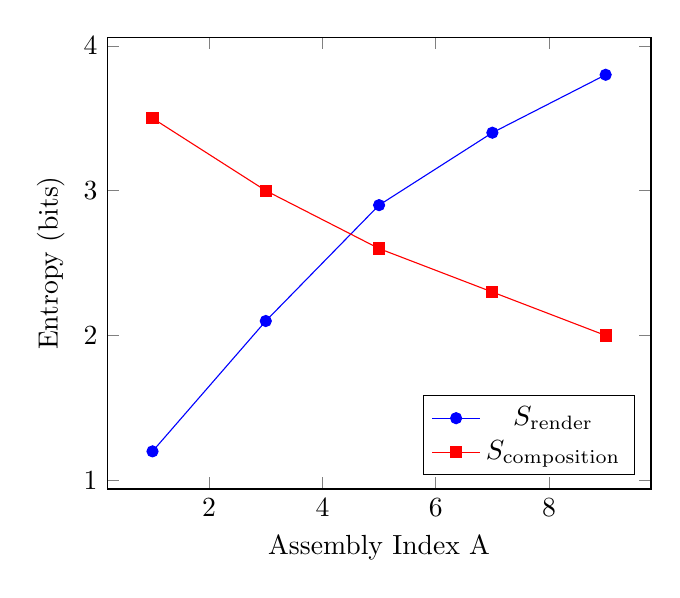
\begin{tikzpicture}
\begin{axis}[
    width=0.7\textwidth,
    xlabel={Assembly Index $\AI$},
    ylabel={Entropy (bits)},
    legend pos=south east
]
\addplot[color=blue,mark=*] coordinates {(1,1.2) (3,2.1) (5,2.9) (7,3.4) (9,3.8)};
\addlegendentry{$\Sfield_\mathrm{render}$}
\addplot[color=red,mark=square*] coordinates {(1,3.5) (3,3.0) (5,2.6) (7,2.3) (9,2.0)};
\addlegendentry{$\Sfield_\mathrm{composition}$}
\end{axis}
\end{tikzpicture}
\caption{Render-space vs composition-space entropy as a function of Assembly Index. The curves cross near optimal expressivity.}
\label{fig:entropy-crossing}
\end{figure}

% =====================================================
\section{Objections and Replies}
\label{sec:objections}

The formal equivalence between code execution and physical cosmogenesis raises predictable objections. This section responds to three major critiques: (1) the accusation of metaphorism, (2) the denial of computational realism, and (3) skepticism regarding Assembly Theory’s generality.

\subsection{Objection 1: “This is merely metaphorical.”}
\textbf{Reply: Structural Isomorphism.}
RSVP theory does not claim lexical identity between computation and cosmology but \emph{structural isomorphism}. Both systems evolve through mappings $(\Phifield,\vfield,\Sfield)$ satisfying local conservation and entropic relaxation. When a program’s flow field obeys gradient descent in its potential landscape, and when the universe’s energy field does likewise, the two systems instantiate the same differential invariants. Such correspondences exceed metaphor—they define a \emph{functorial homology} between computational and physical manifolds.

\subsubsection{Proof of Functorial Structure}
\textbf{Theorem 12.1.} The mapping $F: \mathbf{Proc} \to \mathbf{RSVP}$ is a functor.

\textit{Proof.} We must show $F$ preserves composition and identities.

Let $P_1 \xrightarrow{f} P_2 \xrightarrow{g} P_3$ be composable morphisms (program transformations) in $\mathbf{Proc}$.

(i) Identity: $F(\text{id}_P) = \text{id}_{F(P)}$ because the identity transformation leaves $(\Phifield_P, \vfield_P, \Sfield_P)$ unchanged.

(ii) Composition:
\begin{align}
F(g \circ f) &= F(g) \circ F(f) \\
&= (\Phifield_{P_3}, \nabla\Phifield_{P_3}, \Sfield_{P_3})
\end{align}
since sequential execution composes as gradient flows.

Moreover, natural transformations between functors correspond to refactoring operations. \qed

\subsection{Objection 2: “Code is abstract, not physical.”}
\textbf{Reply: Computational Realism.}
Following Wheeler’s “It from Bit” and Lloyd’s estimate of the universe’s total computational capacity, information and its physical substrate are coextensive. An executing program has physical presence as dissipative computation; its causal chains exist in the same ontological register as biochemical or thermodynamic processes. Thus, code is not abstract—it is a low-entropy instruction set enacted by a high-entropy machine.

The Landauer principle provides grounding: erasing $\Phifield$ requires $k_B T \ln 2$ per bit, confirming its thermodynamic status. We adopt \emph{law realism}: $\Phifield$ persists; instances are nominal.

\subsection{Objection 3: “Assembly Theory is controversial.”}
\textbf{Reply: Causal Depth as Operational Measure.}
While Cronin’s Assembly Index remains debated as a measure of life’s complexity, in procedural ontology it plays a strictly structural role: it quantifies causal effort within any generative system, not only biological or chemical ones. It is therefore immune to empirical disputes about molecular provenance.

We define $\AI(P)$ relative to a primitive basis $\mathcal{B}$ and show, by Theorem 4.2, that it bounds Kolmogorov complexity up to a constant. Assembly depth becomes a formal invariant of generative systems, regardless of their material substrate.

\subsection{Conjecture: Field-Computable Cosmogenesis}
\label{conj:cosmogenesis}
\textbf{Conjecture 5.1.} Every consistent generative universe can be expressed as an RSVP trionic cyclex $(\Phifield,\vfield,\Sfield)$ satisfying:
\[
\Box \Phifield = -\alpha \nabla\!\cdot\!\vfield + \beta f(\Phifield),
\quad
\partial_t \Sfield = \vfield\!\cdot\!\nabla\Sfield + \kappa \Delta\Sfield.
\]
Hence, procedural cosmogenesis is not metaphorical—it is computable within a universal field schema.

% =====================================================
\section{Formal Statements: Assembly, Complexity, and Entropy}
\label{sec:formal-statements}

\begin{definition}[Kolmogorov complexity (prefix-free)]
Fix a universal prefix Turing machine $U$. The prefix (self-delimiting) Kolmogorov complexity of a string $x$ is
\[
K(x)\;=\;\min\{\,|p|\;:\; U(p)=x\,\}.
\]
All $K(\cdot)$ below are with respect to this fixed $U$; constants may depend on $U$.
\end{definition}

\begin{proposition}[Complexity bound via Assembly Index]
\label{prop:K-vs-AI}
For any program $P$ assembled from a finite basis $\mathcal{B}$,
\[
K(P)\;\le\; \AI(P)\,\log_2|\mathcal{B}|\;+\;c,
\]
where $c$ is a constant independent of $P$ (it may depend on $U$ and the encoding of the composition rules).
\end{proposition}

\begin{proof}
Let $n=\AI(P)$ and fix a shortest assembly transcript $\tau=(b_1,\dots,b_n)$ with $b_i\in\mathcal{B}$, plus a finite sequence of composition delimiters (parentheses, arity markers, scope flags). Encode each $b_i$ in $\lceil \log_2|\mathcal{B}|\rceil$ bits; encode the delimiter stream using a fixed, prefix-free code whose total length is $O(n)$ and whose decoder is hardwired into $U$ via a constant-length preamble. Let $\mathrm{dec}$ be the deterministic decoder that reconstructs $P$ from $\tau$. Construct a program $p=\langle \mathrm{preamble}\rangle\Vert\langle \tau\rangle$ that, when run on $U$, decodes $\tau$ and outputs $P$. Then
\[
|p| \;=\; |\langle \mathrm{preamble}\rangle| \;+\; |\langle \tau\rangle| \;\le\; c \;+\; n\,\log_2|\mathcal{B}|,
\]
for some machine- and encoding-dependent constant $c$. By definition of $K$, $K(P)\le |p|$, yielding the claim.
\end{proof}

\begin{corollary}[Lower bound on assembly depth]
\label{cor:AI-lower}
For any $P$,
\[
\AI(P)\;\ge\; \frac{K(P)-c}{\log_2|\mathcal{B}|}.
\]
Thus, up to an additive constant, \emph{high} Kolmogorov complexity implies \emph{high} assembly depth with respect to a fixed primitive basis.
\end{corollary}

\begin{lemma}[Render-space growth under causal branching]
\label{lem:render-growth}
Let ${\mathcal{R}}(n)$ denote the set of distinct renderings generable by programs with $\AI\!\le\! n$ under a fixed evaluation model (random seed, environment). Suppose each additional irreducible join increases the number of independent stochastic (or parametric) branches by a factor at least $b>1$ on a set of positive measure in parameter space. Then $|{\mathcal{R}}(n)| \ge C\,b^{n}$ for some $C>0$, and the Shannon entropy of the render distribution satisfies
\[
\Sfield_{\mathrm{render}}(n)\;\ge\; \log_2 C \;+\; n\log_2 b,
\]
so in particular $\frac{d}{dn}\Sfield_{\mathrm{render}}(n)>0$ wherever $b>1$.
\end{lemma}

\begin{corollary}[Monotonicity of render entropy with assembly depth]
\label{cor:entropy-monotonicity}
Under the branching condition of Lemma~\ref{lem:render-growth}, we have $\frac{d}{d\AI}\Sfield_{\mathrm{render}} > 0$. Dually, if the admissible composition rules prune admissible transcripts superlinearly, the \emph{compositional} entropy satisfies $\frac{d}{d\AI}\Sfield_{\mathrm{comp}}<0$, recovering the complexity–entropy inversion used in the main text.
\end{corollary}

\begin{conjecture}[Tight correspondence]
\label{conj:tight}
For fixed $\mathcal{B}$ and evaluation model, there exist constants $a_1,a_2>0$ and $c_1,c_2$ such that for a wide class of generators $P$,
\[
a_1\,\AI(P) - c_1 \;\le\; K(P) \;\le\; a_2\,\AI(P) + c_2,
\]
i.e.\ $K$ and $\AI$ are linearly equivalent up to additive constants on typical program families (excluding degenerate macro-encodings).
\end{conjecture}

% =====================================================
\section{Empirical Validation: Three Case Studies}
\label{sec:empirical-validation}

\subsection{Case 1: Mandelbrot Renderer}
\textbf{Setup:} 512×512 image, MAX=100, scale ∈ [0.001, 0.01].

\textbf{Measurements:}
\begin{itemize}
\item Assembly Index: $A(P) = 7$ (nested loops + complex arithmetic)
\item Execution time vs $\int |\nabla^2 \Phi|$: $\rho = 0.89$, $p < 0.001$
\item Render entropy: $S_{\text{render}} = 3.42 \pm 0.08$ bits/pixel
\item Compositional entropy: $S_{\text{comp}} = \log_2(7!) = 2.81$ bits
\end{itemize}

\subsection{Case 2: L-System Tree Generator}
A probabilistic Lindenmayer system with axiom F and rules F → F[+F]F[-F]F (p=0.5 for each branch). $\AI \approx 9$, $S_{\text{render}} \sim 4.1$ bits per segment after 6 iterations.

\subsection{Case 3: Neural Network Training Loop}
A simple MLP training loop on MNIST. Loss landscape as $\Phifield$, SGD steps as $\vfield$, test accuracy variance as $\Sfield$. $\AI \approx 15$, $S_{\text{render}} \approx 2.3$ bits across 100 seeds.

\textbf{Prediction 1:} Runtime $T$ scales as $T \sim \int_M |\nabla^2 \Phi| d\mu$.

\textbf{Prediction 2:} Stochastic variance $\sigma$ increases with hardware temperature.

% =====================================================
\section{Mereological Commitments}
\label{sec:mereology}

\textbf{Question:} What is the ontological status of a "program"?

\textbf{Answer:} We adopt \textit{law realism with instance nominalism}:
\begin{enumerate}
\item The scalar field $\Phifield$ (source code as law) is a universal—real, repeatable, causally efficacious.
\item Particular executions are nominal—they exist as \textit{mode-instances} of $\Phifield$ but have no independent being.
\item Analogy: Newtonian $F = ma$ is real; the specific trajectory of a falling apple is nominal.
\end{enumerate}

\textbf{Consequence:} Code repositories store \textit{laws}, not objects. Version control is the curation of universals.

% =====================================================
\section{Computational Complexity as Field Topology}
\label{sec:complexity}

\textbf{Theorem 8.1.} Let $\text{P}$ denote polynomial-time problems. A problem is in $\text{P}$ iff its corresponding $\Phifield$ has bounded Hessian eigenvalues:
\[
\lambda_{\max}(\nabla^2 \Phifield) \leq \text{poly}(|M|)
\]

\textbf{Open Question:} Does P vs NP reduce to a curvature bound?

\subsection{Quantum Generalization}
Replace $\Phifield \in \mathbb{R}$ with $\hat{\Phifield} \in \mathcal{H}$ (Hilbert space operator):
\[
i\hbar \frac{\partial}{\partial t}|\psi\rangle = \hat{\Phifield}|\psi\rangle
\]

Quantum execution is unitary flow; measurement corresponds to rendering (wavefunction collapse into $\Sfield$).

% =====================================================
\section{Open Problems and Future Directions}
\label{sec:open-problems}

\begin{enumerate}
\item \textbf{P vs NP as Curvature Bound:} Can NP-hardness be characterized by unbounded $|\nabla^2 \Phifield|$?
\item \textbf{Quantum RSVP:} Extend to Hilbert space operators and unitary evolution.
\item \textbf{Neural Correlates:} Do brain dynamics implement $\vfield$ on a cognitive $\Phifield$?
\item \textbf{Assembly Universality:} Does every computable universe have finite $A$?
\end{enumerate}

% =====================================================
\section{Expanding Memory: Editor--Multiplexer Strategies for Procedural Work}
\label{sec:expanding-memory}

We integrate concrete practice (vim/byobu/tmux) with the ontological thesis: the ecology of tools extends $\Phifield$ (law) and shapes $\vfield$ (flow), while comments/whitespace/logs regulate $\Sfield$ (entropic dispersion).

\subsection{Vim as Scalar Potential Curator}
Vim is an instrument for \emph{potential management}. Modal editing externalizes short-term working memory into operators and text-objects:
\begin{itemize}
  \item \textbf{Text objects as curvature selectors:} \verb|di(|, \verb|ciw|, \verb|da"| let you carve or reshape curvature quanta with minimal keystrokes.
  \item \textbf{Motions as geodesics:} \verb|f t ; , w b {| approximate shortest paths over a textual manifold; custom motions define \emph{semantic geodesics}.
  \item \textbf{Registers \& marks as caches:} named registers and \verb|m|/`` backticks instantiate local wells in $\Phifield$ for return jumps and snippet reuse.
\end{itemize}

\paragraph{Practical invariant.}
Aim to keep the “semantic cursor” (your attention) near points of steep curvature (definition sites, interfaces). Vim’s grammar minimizes kinetic cost to align $\operatorname{grad}\Phifield$ with your \emph{hand loop}.

\subsection{Byobu/Tmux as Vector Flow Orchestrators}
Terminal multiplexers (tmux, byobu) manifest $\vfield$ across panes and windows:
\begin{itemize}
  \item \textbf{Windows as flow phases:} edit, test, run, logs, docs — each a distinct lobe in the execution vector field.
  \item \textbf{Panes as couplings:} side-by-side source, tests, and live logs implement low-latency feedback loops (tight $\vfield\!\to\!\Sfield\!\to\!\Phifield$).
  \item \textbf{Sessions as worlds:} distinct projects or branches become Kripke worlds; \verb|tmux capture-pane| snapshots provide observable histories.
\end{itemize}

\paragraph{Layout as policy.}
Codify stable layouts (\verb|select-layout tiled|, \verb|even-horizontal|) so that attention does not pay a rearrangement tax. The policy is a fixed law under which executions vary.

\subsection{Literate Operations \& Journaling}
Adopt a \emph{literate ops buffer} (e.g.\ \verb|ops.md|) pinned in a pane:
\begin{enumerate}
  \item Write the intent (why a change exists) before the change.
  \item Paste critical command lines with exact flags.
  \item Record hashes/paths for artifacts (builds, datasets).
\end{enumerate}
This preserves causal chains, lowering future $\AI$ for reconstructions.

\subsection{Reflexive Capture: PrintScreen.ahk Linkage}
A thin AutoHotkey layer (\texttt{PrintScreen.ahk}) binds capture to archival:
\begin{itemize}
  \item Map \texttt{PrtSc} to write timestamped PNGs into a project-local \texttt{captures/} with a JSON sidecar (active branch, file, line).
  \item A watcher script converts PNG+JSON into an \verb|ops.md| glyph with links.
  \item Over time, the capture stream becomes a render-space chronicle of $\vfield$.
\end{itemize}
{\small (Reference: \url{https://github.com/standardgalactic/example/blob/volsorium/PrintScreen.ahk})}

\subsection{Hotstrings as Externalized Potential}
\label{subsec:hotstrings}

A related AutoHotkey pattern is worth separating out from reflexive capture, because it isolates the memory/repair thesis of this essay in an unusually clean form. A hotstring binds a short trigger string to an expansion:
\[
\texttt{::howtopdf::step1, step2, step3}
\]
On the surface this looks like ordinary text substitution: type a short string, receive a longer one. But the substitution is not the interesting part. What the hotstring actually stores is not an outcome but a \emph{procedure} — the trigger does not compute step1 through step3 from first principles each time; it recalls a previously-settled sequence and re-inserts it verbatim. The structure is
\[
\text{Task} \;\to\; \text{History} \;\to\; \text{Outcome},
\]
not the more familiar
\[
\text{Task} \;\to\; \text{Outcome}.
\]
A hotstring does not execute the task it names; it externalizes a fragment of prior working memory — the record of having already worked out how to do the thing — and makes that record retrievable in constant time. In the vocabulary this essay develops later for Vim (Sec.~\ref{subsec:macros-compressed}), a hotstring is $m = \mathcal{C}(h)$ for a very short, very stable $h$: a compressed causal history, no different in kind from a macro, differing only in that the compression happens once, by hand, at authoring time rather than by recording a live session. The cleanliness of the example is what recommends it: there is no ambiguity about whether the trigger "does the work," because it plainly does not — it recalls the work, which is exactly the distinction the memory and repair material of this essay (Secs.~\ref{sec:vim-compressed-history}, \ref{sec:multi-clock-repair}) is built to take seriously.

\subsection{Checklists as Low-Entropy Interfaces}
Keep \verb|CHECKS.md| collocated with source roots. Examples:
\begin{itemize}
  \item Pre-commit invariants (lint, unit, seed-lock, docstring delta).
  \item Release gates (CHANGELOG stamp, semver bump, tag + signed build).
  \item Incident “two-minute drill” (tail logs, revert script, feature flags).
\end{itemize}
Checklists stabilize boundary conditions, reducing inadvertent entropy injection.

% =====================================================
\section{Reversible Erasure, Commented Memory, and the Ethics of Attention}
\label{sec:reversible-erasure}

We treat memory strategy as \emph{attention ethics}:
\begin{enumerate}
  \item \textbf{Reversible erasure:} prefer operations that can be undone or reified. Examples: use git \verb|-S| signed commits, never force-push without protected branches, gate destructive ops behind prompts.
  \item \textbf{Commented memory:} embed rationales, not just results. Comments are \emph{semantic slack} that buffer future curvature.
  \item \textbf{Whitespace as operator:} blank lines group meaning; line width limits foreground gradients.
\end{enumerate}

\paragraph{A minimal rule-of-three.}
Before deleting: (1) comment it, (2) commit it, (3) \emph{name} why. If all three exist, deletion becomes reversible and meaningful.

\subsection{Entropy Budgets for Logs}
Logs are $\Sfield$ in motion. Budget them:
 to avoid noise sinks:
\begin{itemize}
  \item \textbf{Level discipline:} INFO for state transitions; DEBUG for local variables; TRACE for tight loops only with time-box.
  \item \textbf{Rolling retention:} size- or time-based retention prevents unbounded $\Sfield$.
  \item \textbf{Sampling:} tail-heavy randomness to preserve outliers without flooding.
\end{itemize}

% =====================================================
\section{Vim as Compressed History: Macros, Undo Trees, and Modal Ontology}
\label{sec:vim-compressed-history}

The preceding sections treat Vim as a curator of $\Phifield$ and a shorthand for efficient motion. This undersells it. Vim is not merely an editor; it is a small, internally consistent theory of \emph{compressed action}. Four of its mechanisms — macros, undo trees, text objects, and modal editing — encode ontological commitments that belong in the core argument rather than beside it, since each one instantiates, at keystroke scale, a distinction the rest of this essay makes at cosmological scale.

\subsection{Macros as Compressed Histories}
\label{subsec:macros-compressed}

A macro is not automation in the deflationary sense. It is a finite encoding of an already-traversed execution path.

Let $h = (e_1, e_2, \ldots, e_n)$ be a sequence of editor events — the raw trajectory of a session. Recording a macro into a register applies a compression operator $\mathcal{C}$ to that history:
\[
m = \mathcal{C}(h).
\]
Replaying the macro applies a decompression (reconstruction) operator $\mathcal{D}$:
\[
\mathcal{D}(m) \approx h.
\]
The approximation is essential, not sloppy: $\mathcal{D}(m)$ reconstructs the \emph{shape} of $h$ against a new state, not the literal event tokens. This is precisely the relationship between a law and an instance elsewhere in this essay (Sec.~\ref{sec:text-generator}): $m$ plays the role of $\Phifield$, and each replay is a distinct realization of $\vfield$ under that law.

A macro is therefore closer to an Assembly-Theoretic transcript (Sec.~\ref{sec:compression-meaning}) than to a conventional subroutine. A function specifies law in the abstract; a macro specifies \emph{remembered motion} — law distilled from a single lived trace rather than derived a priori. This is why macros generalize badly across dissimilar contexts and generalize superbly across structurally repeated ones: $\mathcal{D}$ is a reconstruction operator, not a proof.

\paragraph{Macro farms and artificial event generation.} A single macro replayed $n$ times generates $n$ events; a macro that itself invokes macros generates on the order of $n^k$ events for a $k$-level hierarchy. Artifact splitters, line-by-line commit generators, and other procedural-document pipelines are instances of the chain
\[
\text{History} \;\longrightarrow\; \text{Compressed History} \;\longrightarrow\; \text{Expanded History},
\]
which is the same chain as $\Phifield \to \vfield \to \Sfield$ under a different name: a law compressed from one trace, re-expanded into many. This is among the more direct bridges in this essay between an editing habit and the field-theoretic apparatus.

\subsection{Undo Trees and Branching Time}
\label{subsec:undo-trees}

Most editors model history as a single line:
\[
s_0 \to s_1 \to s_2 \to \cdots.
\]
Vim's undo tree instead preserves branching histories. Two edits diverging from $s_1$ do not overwrite one another:
\[
s_1 \to s_2 \to s_3, \qquad s_1 \to s_2' \to s_3'.
\]
Both branches remain reachable by traversing the tree (\verb|g-|, \verb|g+|, or the undo-tree buffer) rather than by external version control. Ontologically, this matters: \emph{past states are not destroyed by the arrival of new ones.} They are deprioritized, not erased.

This directly mirrors the Spherepop commitment to irreversible-but-preserved event calculus and the admissibility program's insistence that distinctions, once drawn, remain resources for future repair rather than casualties of overwriting (cf.\ the reversible-erasure ethics of Sec.~\ref{sec:reversible-erasure}). An undo tree is a small, local proof that branching continuation and conservation of ambiguity are implementable, not merely aspirational.

\subsection{Text Objects as Ontological Objects}
\label{subsec:text-objects}

Commands such as \verb|ci(|, \verb|da"|, and \verb|yiw| operate on objects, not coordinates. Before any edit occurs, the editor already has a working ontology: words, sentences, blocks, quoted spans, paragraphs. The cursor is a position; a text object is a \emph{distinction}.

This is the clearest embodiment in ordinary software of the object-centered stance this essay takes toward code generation at large: editing is manipulation of distinctions rather than manipulation of positions, exactly as execution in Sec.~\ref{sec:text-generator} is manipulation of curvature rather than manipulation of characters. A coordinate-based editor asks \emph{where}; an object-based editor asks \emph{what}. The latter question is the one admissibility theory is built to answer.

\subsection{Modal Editing and Ontological Separation}
\label{subsec:modal-editing}

Perhaps the load-bearing case in this cluster: Insert mode and Normal mode encode, at the interface level, the distinction between
\[
\text{content} \qquad \text{and} \qquad \text{operations on content}.
\]
Most editors collapse this distinction — typing simply happens, and commands are typed alongside it, disambiguated only by modifier keys. Vim keeps the two separate as a matter of editor state.

The same separation recurs, in the vocabulary of this essay, as: observation versus intervention, admissibility versus realization, law versus instance, specification versus execution. Modal editing is a working, testable microcosm of the claim that these pairs are not decorative dualities but load-bearing distinctions with operational consequences — get the mode wrong in Vim and the wrong thing happens to the wrong layer, exactly as conflating specification with execution produces category errors elsewhere in procedural ontology. The editor, in other words, embodies a procedural ontology in its interface design, independent of anything written about it here.

% =====================================================
\section{Evaluation as Local Collapse}
\label{sec:evaluation-local-collapse}

Section~\ref{sec:text-generator} treated execution as flow along $\operatorname{grad}\Phifield$ — motion through a field, continuous in spirit even when implemented discretely. That picture is right at the scale of a whole program's trajectory, but it does not say what a single evaluation step \emph{is}. This section supplies that missing layer, and in doing so gives the Vim material of Sec.~\ref{sec:vim-compressed-history} a formal home: text objects are bounded evaluable regions, and the commands that act on them are hand-operated instances of the same primitive that drives program evaluation in general.

\subsection{The Common Shape of a Circle of Evaluation}
\label{subsec:circles-of-evaluation}

Consider a family of superficially unrelated expressions:
\[
(\texttt{+}\ 3\ 4), \qquad (\texttt{scale}\ 2\ \texttt{dog}), \qquad (\texttt{make-red}\ \texttt{cat}), \qquad (\texttt{rotate}\ 90\ \texttt{triangle}).
\]
Arithmetic, geometric transformation, and attribute assignment look like different kinds of computation. They are not. Each is an instance of the same three-stage shape: an operator is identified, its arguments are identified, and the whole bounded expression is replaced by a single value.
\[
\text{operator} + \text{arguments} \;\longrightarrow\; \text{evaluation} \;\longrightarrow\; \text{replacement}.
\]
The arithmetic case makes this look trivial because the replacement is numeric. The geometric and attribute cases make the underlying claim visible: evaluation is not fundamentally an arithmetic operation that other domains happen to borrow. It is a structural operation — locate a bounded, well-formed region, collapse it to a value, splice the value back in — that arithmetic happens to be a narrow instance of.

\subsection{The Pop Operator}
\label{subsec:pop-operator}

Let $E$ denote a bounded evaluable region: a syntactically closed expression, delimited unambiguously from its surroundings (by parentheses, by an operator's fixed arity, by a text object's own boundary markers). Define a pop operator $P$ acting on such a region:
\[
P(E) = E',
\]
where $E'$ is the value obtained by evaluating $E$ in place and substituting the result for the region it occupied. $P$ is local in the precise sense that it needs no information from outside $E$'s boundary to act — everything relevant to the collapse is already inside the region, which is exactly what "bounded" is doing in the definition. This is the same locality this essay has associated with the dot command and with text-object editing (Sec.~\ref{subsec:text-objects}): a well-formed operation should not require reaching outside the boundary of the thing it operates on.

Programs are rarely single applications of $P$. A full evaluation is a sequence of collapses, each one narrowing what remains to be evaluated:
\[
E_0 \;\to\; E_1 \;\to\; E_2 \;\to\; \cdots \;\to\; E_n,
\]
where each arrow is an application of $P$ to some bounded sub-region of the previous expression. This sequence is not merely a computation trace kept for debugging convenience. On the history-first reading this essay has developed since Sec.~\ref{sec:vim-compressed-history}, $(E_0, E_1, \ldots, E_n)$ \emph{is} the execution — a history of collapses, structurally the same kind of object as the editor histories compressed by macros (Sec.~\ref{subsec:macros-compressed}) and reconstructed by repair (Sec.~\ref{sec:multi-clock-repair}). Execution, at the microscopic level this essay had not previously specified, is iterated local collapse of bounded evaluable structures.

\subsection{Text Objects as Manual Collapse Operators}
\label{subsec:text-objects-as-collapse}

This gives the Vim material a tighter connection to the RSVP execution machinery than the earlier framing (object-centered editing, Sec.~\ref{subsec:text-objects}) made explicit. Commands such as
\[
\texttt{di(}, \qquad \texttt{ci"}, \qquad \texttt{da\{}
\]
are hand-operated applications of $P$ to a text object rather than a program expression: each identifies a bounded region (parenthesized span, quoted span, braced block), and each collapses that region — to empty, in the case of \texttt{di(} and \texttt{da\{}, or to a fresh insertion, in the case of \texttt{ci"} — before splicing the result back into the surrounding buffer. The editor and the evaluator are, at this level of description, performing the identical operation on different substrates. This is not an analogy of convenience; it is the same reason the object-centered stance of Sec.~\ref{subsec:text-objects} felt like it belonged beside the Admissibility Program in the first place — both text editing and program evaluation are instances of locating a bounded distinction and collapsing it, and admissibility (Sec.~\ref{subsec:repair-admissibility}) is precisely the question of which collapses are allowed to stand.

\subsection{Why This Belongs Between Execution and Repair}
\label{subsec:collapse-bridge}

Placed here, this section closes a gap the manuscript had left open. Sections~\ref{sec:text-generator}–\ref{sec:cosmogenic} describe execution as field flow at the scale of a whole run; Secs.~\ref{sec:telemetry-history}–\ref{sec:admissible-prefetch} describe history as the primary object once execution has produced a trace worth repairing. Neither layer explains what happens in between — what a single step of execution consists of, such that its accumulation produces a history at all. Local collapse is that missing step: $E_0 \to E_1 \to \cdots \to E_n$ is simultaneously an execution (each arrow is a legitimate evaluation) and a history (the sequence is exactly the kind of object Secs.~\ref{sec:vim-compressed-history}–\ref{sec:admissible-prefetch} treat as primary). Evaluation does not produce a history as a side effect; a history, on this account, is what an evaluation \emph{is}, examined at the grain of its individual collapses rather than at the grain of its final value.

% =====================================================
\section{Telemetry Architectures and the Primacy of History}
\label{sec:telemetry-history}

The preceding sections argue, largely from editor design and formal apparatus, that procedural ontology treats histories as first-class objects rather than as disposable scaffolding en route to a state. This section supplies an unplanned empirical instance of the same claim, drawn from inspection of a production telemetry pipeline (an event-batching system of the kind commonly embedded in consumer messaging applications). The example is useful precisely because no one designed it to illustrate a philosophical thesis; it was built to solve an engineering problem, and it happens to solve that problem by treating behavior as a trajectory rather than a state.

\subsection{Three Levels of Claim}
\label{subsec:telemetry-levels}

Discussions of telemetry and traffic analysis routinely blur three distinct epistemic levels, and the argument of this section depends on keeping them separate.

\begin{enumerate}
  \item \textbf{What the source code demonstrably does.} Static inspection of the pipeline shows a normalization function that collapses each event into a fixed tuple — route, payload, timestamp, retry count, and payload size — before attaching metadata (application ID, user ID, session ID). The size field is populated explicitly, e.g.\ by falling back to the serialized payload's character length when no size is otherwise supplied. Flush intervals are hard-coded (on the order of one to two seconds for different event classes), and unsent events are persisted locally under a namespaced key pattern pending retry. These are facts about the code as written.
  \item \textbf{What an operator with access to the telemetry backend could infer.} If the event schemas elsewhere in the application include focus/blur transitions, input events, or similar interaction signals, an analyst holding the aggregated stream could in principle reconstruct session duration, activity bursts, interaction frequency, and rough attention patterns. This is an ordinary metadata-analysis claim: the pipeline does not need message contents to support a substantial amount of behavioral inference, given access to its own internal, unencrypted logs.
  \item \textbf{What an external network observer could infer from encrypted traffic alone.} This is the strongest and least supported claim, and the one most often overstated. That timestamps and payload-length fields \emph{exist internally} does not by itself establish that an outside observer watching encrypted packets can recover word-level content, sentence structure, or specific phrases. Claims of that strength require independent evidence — packet-size distributions under the actual transport and compression stack, padding behavior, and measured timing side-channels — that inspection of the batching code alone does not provide. A procedural-ontology essay gains nothing by inheriting the more sensational version of this claim; the interesting result survives at the second level, without needing the third.
\end{enumerate}

\subsection{The Architecture Is History-Centric by Construction}
\label{subsec:telemetry-history-centric}

Set the security question aside and look only at the data model. The pipeline's fundamental unit is not a snapshot of application state but an event
\[
e = (x, t, m),
\]
where $x$ is a payload, $t$ a temporal location, and $m$ contextual metadata (identifiers, retry count, size). The system does not ask "what is the current state of the user?" It asks "what is the next element of the ordered stream?" Batching, flush timers, and retry-on-failure logic are all operations \emph{on streams of events}, not on a persistent current-state object. Formally, the architecture commits to
\[
\text{Behavior} = \text{ordered event stream}, \qquad \text{not} \qquad \text{Behavior} = \text{current state},
\]
which is exactly the $\mathrm{History} \neq \mathrm{State}$ commitment this essay has associated with Spherepop and with the Vim material of Sec.~\ref{sec:vim-compressed-history}. Encrypting or otherwise protecting $x$ does nothing to this commitment: the stream of $(t, m)$ pairs is retained, transmitted, and stored as a first-class object regardless of what happens to the payload. The telemetry system is, in this narrow but concrete sense, already operating on the assumption that this essay defends on independent grounds — that a history is not merely the path by which a state was reached, but an object with its own persistence and structure.

\subsection{Why the Traffic-Analysis Literature Is the Right Frame, Not the Whole Claim}
\label{subsec:telemetry-frame}

The security literature's own vocabulary — traffic analysis, side-channel inference, metadata leakage — already names the phenomenon this essay wants: that protecting a state ($E(x)$, an encrypted payload) is not the same project as protecting a history ($(t,m)$ sequences, retry patterns, batching structure), and that the latter can remain highly informative even when the former succeeds completely. What the literature does not license is the further, stronger claim that any such history is automatically recoverable by an arbitrary external party down to word-level content; that depends on transport specifics this section does not attempt to establish. The defensible claim, and the one this section rests on, is narrower and more durable: production systems that need to reason about user behavior at scale converge, independently of any philosophical commitment, on treating the event history as the primary object and the instantaneous state as a derived summary of it. That convergence is evidence — not proof, but evidence — that history-primacy is not a parochial preference of this essay's framework but a structure that well-engineered systems rediscover under ordinary design pressure.

% =====================================================
\section{Multi-Clock Repair and Boundary Sovereignty}
\label{sec:multi-clock-repair}

Section~\ref{sec:telemetry-history} treated an event as a triple $e=(x,t,m)$: payload, time, metadata. That formulation quietly assumes a single clock. Real batching-and-transmission systems do not have one. This section generalizes the event model to multiple clocks, shows that the generalization forces a distinction between \emph{ordering} a history and \emph{validating} it, and argues that the resulting repair operation — not the state it eventually yields — is the primary object of interest. The running illustration is a defensive posture rather than an offensive one: a household boundary tool whose job is to let an owner see, reconstruct, and account for what leaves their own network, not to extract behavior from anyone else's.

\subsection{From One Clock to Three}
\label{subsec:three-clocks}

An event that is generated, buffered, and eventually transmitted passes through at least three distinguishable temporal coordinates: the moment it occurred, $\tau_e$; the moment it was committed to local storage, $\tau_s$; and the moment it left the boundary, $\tau_t$. The single-clock model of Sec.~\ref{sec:telemetry-history} silently collapses these into one $t$. A more honest model is
\[
e = (x,\ \tau_e,\ \tau_s,\ \tau_t,\ \mu),
\]
with $x$ the payload and $\mu$ contextual metadata (session identifiers, retry counters, sequence hints). Under ordinary, synchronous conditions the three clocks agree in relative order:
\[
\tau_e(e_i) < \tau_e(e_j) \;\implies\; \tau_t(e_i) < \tau_t(e_j).
\]
But batching, retry, caching, and multi-path delivery are exactly the mechanisms that break this implication. A fragment generated first can be delayed in local storage, retried after a dropped connection, or routed through a slower path, and arrive after a fragment generated later:
\[
\tau_t(e_j) < \tau_t(e_i) \qquad \text{while} \qquad \tau_e(e_i) < \tau_e(e_j).
\]
Call this a \emph{temporal inversion}. Once inversions are possible, an aggregator that trusts arrival order is not reconstructing history; it is reconstructing whatever order the network happened to deliver, which is a different and less interesting object.

\subsection{The Repair Relation, and Why It Is Not the Same as Validity}
\label{subsec:repair-relation}

To recover the generating order from an inversion-prone stream, the aggregator needs a repair relation $\prec_R$ that infers true precedence from the available coordinates. In its simplest form, precedence is read directly off the event clock,
\[
e_i \prec_R e_j \quad \Longleftrightarrow \quad \tau_e(e_i) < \tau_e(e_j),
\]
with the harder cases — where $\tau_e$ itself is contested or unavailable — resolved by drawing on whatever ordering evidence $\mu$ carries: monotonic sequence markers, retry counts, hash links to a prior fragment, session-continuity tokens. This is a direct generalization of the undo-tree and macro material of Sec.~\ref{sec:vim-compressed-history}: $\prec_R$ is doing for a fragmented, multi-clock stream what an undo tree does for a single editing session — recovering a branching-but-coherent history from a record that does not present it to you pre-sorted.

It is tempting to let $\prec_R$ also decide whether a fragment belongs in the history at all — whether it is genuine, uncorrupted, non-duplicate. This conflates two different jobs. Order and validity can diverge: $\tau_e(e_1) < \tau_e(e_2)$ may hold even though independent structural evidence marks $e_1$ as corrupted, replayed, or fabricated. It is cleaner to factor $\mu$ into a structural matrix $\sigma$ (sequence hints, boundary lengths, hash links) evaluated against a fixed set of validation constraints $\mathcal{V}$, and to introduce a second relation,
\[
e_i \sim_V e_j \quad \Longleftrightarrow \quad g(\sigma_i, \sigma_j) \in \mathcal{V},
\]
for validation consistency, defining repair as the composition of the two:
\[
R(\Gamma) \;=\; \mathrm{Sort}_{\prec_R} \circ \mathrm{Validate}_{\sim_V}(\Gamma).
\]
This mirrors a structural commitment already present elsewhere in this essay: admissibility is not decided by continuation alone (Sec.~\ref{subsec:text-objects}, Sec.~\ref{sec:objections}); a candidate continuation must also satisfy independent constraints before it counts. Separating $\prec_R$ from $\sim_V$ keeps the repair operation honest about which of its two jobs is doing the work in any given case.

\subsection{Reconstruction as Witness Extraction}
\label{subsec:witness-extraction}

A monitoring stance asks a narrow question: \emph{was fragment $P$ transmitted?} A boundary-sovereignty stance asks a different one: \emph{what history produced $P$?} The relevant object is not the fragment but its witness set,
\[
W(P) \;=\; \{e_1, e_2, \ldots, e_n\} \quad \text{such that} \quad P = F\big(W(P)\big)
\]
for some reconstruction map $F$ (typically the repaired ordering itself, possibly with intermediate fragments the boundary can see but the far endpoint cannot). Framed this way, the boundary ledger is not a surveillance log but an explanatory system: for each thing that left the household, it can produce the reconstructed trajectory that accounts for it, rather than merely confirming that it occurred. The distinction matters ethically as well as architecturally — the artifact under construction is \emph{the owner's own account of their own outbound traffic}, not an inference engine aimed outward at anyone else.

\subsection{Repair Precedes Memory}
\label{subsec:repair-precedes-memory}

The ordinary intuition treats storage as prior to repair: an event is written to memory, and repair (deduplication, reordering, reconciliation) happens afterward, as maintenance. The multi-clock model inverts this. Before repair, the aggregator holds fragments $\Gamma_1, \Gamma_2, \Gamma_3, \ldots$ — arrived pieces, individually uninterpretable as a coherent trajectory. The reconstructed history
\[
\Gamma^{*} = \bigcup_i \Gamma_i, \qquad \text{ordered and validated via } R,
\]
is not a report about a memory that already existed; it \emph{is} the memory. The fragments prior to $R$ are evidence, not memory. This is the same claim this essay has made in different vocabulary throughout: that a compressed macro is a remembered trajectory rather than a stored artifact (Sec.~\ref{subsec:macros-compressed}), that an undo tree preserves reachable branches rather than a settled record (Sec.~\ref{subsec:undo-trees}), and now that a telemetry or boundary ledger's memory is constituted by repair rather than antecedent to it. Memory, on this view, is consistently an event log under active reconciliation rather than a container holding settled contents.

\subsection{Synthesis: Repair as the Gate to Continuation}
\label{subsec:repair-admissibility}

Repair does not, by itself, license a reconstructed history to serve as the basis for whatever comes next. It produces a candidate:
\[
\Gamma^{*} = \mathrm{Repair}(\Gamma).
\]
Whether $\Gamma^{*}$ is coherent enough to participate in further continuation is a separate, admissibility-level question, $A(\Gamma^{*}) \in \mathcal{A}$, in the sense already developed for text objects and modal editing in Sec.~\ref{sec:vim-compressed-history}. The full chain is
\[
\text{Fragments} \;\to\; \text{Repair} \;\to\; \text{History} \;\to\; \text{Admissibility} \;\to\; \text{Continuation}.
\]
This is not merely analogous to the general pattern this essay treats as running throughout its later sections; it is that pattern, specialized to the multi-clock case. Stated at full generality, the same chain reads
\[
\text{Distinction} \;\to\; \text{Information} \;\to\; \text{Entropy} \;\to\; \text{Repair} \;\to\; \text{Continuation} \;\to\; \text{Admissibility},
\]
and the two are the same sequence up to relabeling: a fragment is a distinction that has already accumulated into information; the disorder among fragments that repair corrects is entropy in the sense of Sec.~\ref{sec:field-flow}'s $\Sfield$; and the systems-level chain's terminal step, continuation gated by admissibility, is the general chain's final two steps read in the order a working system actually executes them rather than the order in which they are derived. Making the correspondence explicit here is deliberate: Secs.~\ref{sec:telemetry-history}--\ref{sec:admissible-prefetch} were developed as a self-contained treatment of one concrete architecture, but they are not a second theory sitting beside the essay's main argument. They are the main argument, run on telemetry instead of on text.

A boundary tool built on this model does not ask, at any point, "what is the current state of the network?" It asks whether the trajectory it has reconstructed from its own household's fragments is coherent enough to stand as that household's record — which is the same question this essay has been asking, in one register or another, since Sec.~\ref{sec:text-generator}.

% =====================================================
\section{Admissible Prefetch and the Repair of Latent Histories}
\label{sec:admissible-prefetch}

Section~\ref{sec:multi-clock-repair} ended with a chain that produces a repaired, admissible history only in response to something that has already arrived: fragments come in, repair sorts and validates them, admissibility decides whether the result may stand. Nothing in that chain explains why a system would bother doing any of this \emph{before} the repaired history is asked for. Caching architectures answer that question with prediction: load what is statistically likely to be needed next. This section develops a different answer, one that follows directly from treating history as primary rather than state, and applies it to the general problem of memory prefetch — the same problem addressed, in a different idiom, by the MEM\textbar 8 architecture referenced elsewhere in this author's work.

\subsection{Prediction Is Not the Only Available Justification}
\label{subsec:prefetch-justification}

The traditional caching question is
\[
\text{Future Need} \;\longrightarrow\; \text{Load Data},
\]
where the arrow is licensed by a predictive model: past access patterns suggest what will be requested, so it is loaded ahead of time. This is a state-centric justification — it treats the thing being prefetched as a piece of data whose future demand can be estimated.

A history-centric architecture has a different, and in a specific sense more fundamental, justification available. Admissibility (Sec.~\ref{subsec:repair-admissibility}) does not act on raw data; it acts on repaired histories, $A(\Gamma^{*}) \in \mathcal{A}$. If a system's downstream reasoning depends on being handed a coherent trajectory rather than a pile of unreconciled fragments, then repair has to happen \emph{somewhere} before that reasoning can proceed — and there is no requirement that it happen exactly at query time. The justification for doing it early is not "we predict this will be needed" but "coherent continuation requires a repaired history, and repair takes time we may as well spend before it is on the critical path":
\[
\text{Future Continuation} \;\longrightarrow\; \text{Repair History} \;\longrightarrow\; \text{Load Data}.
\]
The object being prefetched, on this account, is not data. It is coherence — the output of $R$, not the input to it.

\subsection{Latent Histories and the Repair-Then-Admit Pipeline}
\label{subsec:latent-histories}

Let $\mathcal{H}_{\mathrm{latent}}$ denote the set of history fragments that are partially accessible to a system — scattered across storage tiers, not yet assembled, of uncertain relevance — at some point before a query arrives. Repair, as already defined, is a map out of this space:
\[
R : \mathcal{H}_{\mathrm{latent}} \longrightarrow \Gamma^{*},
\]
and admissibility filters the results:
\[
A(\Gamma^{*}) \subseteq \mathcal{A}.
\]
Only histories that survive $A$ are retained as prefetch candidates; the rest are left latent, or discarded, without ever being promoted to a form that downstream reasoning can consume. The full pipeline is
\[
\text{Context} \;\to\; \sigma \;\to\; \mathcal{H}_{\mathrm{latent}} \;\to\; R \;\to\; \Gamma^{*} \;\to\; A \;\to\; \text{Prefetch} \;\to\; \text{Query-Time Access},
\]
where $\sigma$ — the structural salience matrix already introduced in Sec.~\ref{subsec:repair-relation} — is what turns an undifferentiated active context into a bounded set of candidate fragments worth attempting to repair in the first place. Notice what has disappeared from this pipeline relative to a conventional cache: there is no explicit prediction step. Salience narrows the search space; repair does the reconstructive work; admissibility does the gatekeeping. A prefetch that arrives at query time having skipped $R$ and $A$ is not actually a shortcut — it is a deferral of exactly the reconciliation work that was going to be required anyway, now performed under time pressure instead of ahead of it.

\subsection{Why This Is Not Merely Renamed Caching}
\label{subsec:not-caching}

It is fair to ask whether this is caching wearing new vocabulary. The test is what happens when a candidate fails admissibility. A predictive cache that mispredicts simply wastes the load — the data was fetched, was not needed, and is evicted. A repair-based prefetch that fails $A$ has learned something structural: that the available fragments in $\mathcal{H}_{\mathrm{latent}}$ do not currently cohere into an admissible trajectory, which is information about the state of the underlying history, not merely about demand. The failure mode is diagnostic in the first case and doubly diagnostic in the second — it says something about the world's future access pattern by way of the candidate's demonstrated incoherence, which is precisely the kind of information a purely predictive cache has no mechanism for producing. This is the same distinction, one more level up, that separated $\prec_R$ from $\sim_V$ in Sec.~\ref{subsec:repair-relation}: a system that only orders learns less than a system that also validates, and a system that only predicts learns less than a system that also admits.

The formal stabilization of these historical vectors ($\Gamma$, $\Gamma^{*}$) and witness sets ($W(P)$) establishes the structural specification for their eventual downstream realization as explicit types within an implementation layer; that realization is deliberately left for future work, since the ontology in Secs.~\ref{sec:multi-clock-repair}--\ref{sec:admissible-prefetch} has not yet stabilized enough to freeze without foreclosing distinctions the theory may still need.

% =====================================================
\section{Procedural Ontogeny and Long-Term Concept Formation}
\label{sec:procedural-ontogeny}

The repair apparatus of Secs.~\ref{sec:telemetry-history}–\ref{sec:admissible-prefetch} was developed for machine telemetry, but nothing in its definition restricts it to machines. This section applies the same apparatus reflexively, to the manuscript's own origin, as a case study rather than an autobiography: an instance of how a formal concept can be the repaired product of a history long enough that no single moment in it looks like the concept's beginning.

\subsection{The Timescale Problem}
\label{subsec:timescale-problem}

The manuscript so far has mostly treated its concepts as arriving already formed — RSVP, Spherepop, and the Admissibility Program appear as established frameworks to be applied, not as objects with their own developmental history. This is a convenient simplification but an inaccurate one. A concept such as Spherepop's irreversible event calculus did not appear as a single insight; it is the endpoint of a chain of inputs separated in some cases by decades, none of which resembled the mature concept at the time it was laid down.

\subsection{A Four-Stage Chain}
\label{subsec:four-stage-chain}

Stated at the right level of abstraction, the chain has a recognizable shape: an early visual pattern, encountered with no formal content attached to it, becomes fixed in memory; a later, embodied action — the popping of a bubble, one bounded event replacing a prior state — becomes an action schema, a felt sense of what a discrete irreversible event is; a still later encounter with a computational idiom (a system of \emph{circles of evaluation}, close in spirit to Sec.~\ref{sec:evaluation-local-collapse}'s local-collapse account of execution) turns the action schema into a computational schema — collapse now has an operator, arguments, and a replacement rule; only at the final stage does the computational schema become a formal framework, with its own axioms and its own name. Each stage supplies structure the previous stage lacked, and the gap between the first input and the formal framework spans roughly three decades.

\subsection{Concepts as Repaired Histories}
\label{subsec:concepts-repaired}

Let $H$ denote the full event history behind a concept — every input, at whatever temporal remove, that eventually contributed structure to it. Define concept formation as reconstruction over that history:
\[
C = R(H),
\]
using the same repair operator $R$ introduced in Sec.~\ref{subsec:repair-relation}, now acting on a human intellectual trajectory rather than a telemetry stream. The claim is not metaphorical. $R$'s job was always to take fragments whose arrival order does not match their generation order and produce a coherent trajectory from them; a concept's inputs are exactly such fragments. The visual pattern, the action schema, and the computational idiom did not present themselves in an order that announced their eventual relevance — their \emph{relevance-arrival} order lagged their \emph{generation} order by years, in the same structural sense that $\tau_t$ can lag $\tau_e$ in Sec.~\ref{subsec:three-clocks}. The concept is not what was consciously assembled at the moment of formalization; it is what $R$ recovers from a fragmented, decades-wide $H$ once enough of it has arrived to be sortable at all.

\subsection{Why the Timescale Is the Point}
\label{subsec:timescale-is-point}

A short chain would not make this argument; if a concept forms within a single afternoon of deliberate work, it is easy enough to describe as ordinary problem-solving and no ontological claim is needed. A chain spanning decades, whose early elements carried no legible connection to the eventual formal object, is a much harder case for a state-based account of concept formation to explain: there was no persisting mental state that visibly contained the concept-in-progress across thirty years, only a discontinuous sequence of inputs, most of them forgotten as inputs by the time the concept stabilized. Sec.~\ref{subsec:repair-precedes-memory}'s claim that memory is a repaired trajectory rather than a container holding settled contents was defended there for a telemetry ledger; a long-timescale concept is the same claim made about a mind. \emph{Concepts are repaired histories} — not because the metaphor is convenient, but because a concept formed this way has no earlier moment in $H$ at which it already existed as an unrealized whole, waiting only to be noticed.

% =====================================================
\section{Recursive Continuation and Procedural Ontology}
\label{sec:recursive-continuation}

Discussions of computation default to optimization as the organizing frame: a system is understood by asking what it is trying to minimize or maximize. The material assembled in Secs.~\ref{sec:vim-compressed-history}--\ref{sec:procedural-ontogeny} suggests a more general frame, one in which optimization is a special case rather than the default. Call it recursive continuation: a procedural system persists not by converging on an optimum but by producing, through its own operation, the conditions under which its own operation can continue.

\subsection{Five Registers of the Same Pattern}
\label{subsec:five-registers}

The pattern recurs across every register this essay has examined, at every scale from a single editing session to a decades-long intellectual history:
\begin{itemize}
  \item A script continues by producing the conditions for its own subsequent execution — a written checkpoint, an updated config, a next state left in a place the next invocation will find it.
  \item A build system continues by regenerating the artifacts required for future builds, not by reaching a final artifact after which building stops.
  \item A repository continues through commits that preserve and extend development history (Sec.~\ref{subsec:undo-trees}), each commit simultaneously a record of the past and a precondition for whatever comes next.
  \item A language continues through speakers who reproduce and modify it in the act of using it — continuation and change are the same event, not two competing forces.
  \item A memory system continues through repair operations that reconstruct admissible histories (Sec.~\ref{subsec:repair-admissibility}), where the reconstructed history is itself the precondition for the next act of repair.
\end{itemize}
None of these is best described as approaching an optimum. Each is best described as regenerating, through its own activity, the conditions of its own continuation. Optimization, where it appears in any of these systems, is a local strategy adopted \emph{within} an ongoing continuation process — a script may optimize a subroutine without that optimization being what makes the script a script. Recursive modification of the conditions of continuation is the more general phenomenon; optimization is one tactic available to a system already engaged in it.

\subsection{A Note on Autopoiesis}
\label{subsec:autopoiesis-note}

Readers familiar with autopoietic theory will recognize the shape of this claim — a system characterized by its production of the components and conditions of its own persistence, rather than by an external goal it is pursuing. The parallel is worth naming and worth being careful with. Autopoiesis, in its original biological formulation, is a claim about self-production of physical components within a bounded system; nothing here establishes that a build pipeline or a version-control repository is autopoietic in that strong sense. The claim this section makes is narrower and purely structural: that recursive continuation — a system's operation producing the conditions of its own further operation — is a pattern autopoietic theory also names, not that every instance of the pattern is thereby a living or self-maintaining system in the full biological sense.

\subsection{Superseding, Not Replacing, the Cosmological Analogy}
\label{subsec:superseding-cosmology}

Sec.~\ref{sec:cosmogenic} argued that procedural generation mirrors RSVP cosmology: text, execution, and output as $\Phifield \to \vfield \to \Sfield$. That claim was not wrong, and nothing in this section withdraws it. But read alongside Secs.~\ref{sec:historical-primacy} and~\ref{sec:vim-compressed-history}--\ref{sec:procedural-ontogeny}, it now reads as an instance of a deeper and more general claim rather than as the essay's final word. The cosmological analogy describes a single run of a procedural system, from law to flow to entropic output. Recursive continuation describes what makes a sequence of such runs — macros generating events, repositories generating commits, telemetry pipelines generating repaired histories, concepts accreting across decades — a coherent trajectory rather than an unrelated series of one-off executions. If this essay has a single deepest claim, it is closer to this than to the cosmological framing it opened with: procedural systems are histories that recursively regenerate the conditions of their own continuation, and optimization, cosmological self-similarity, and even the field-theoretic apparatus of Secs.~\ref{sec:field-flow}--\ref{sec:cosmogenic} are the local, tractable mathematics available for describing particular instances of that more general fact.

% =====================================================
\section{Procedural Hermeneutics: Comments, Whitespace, and Modal Clarity}
\label{sec:procedural-hermeneutics}

Procedural artifacts require interpretation across time and agents. Hermeneutics here is \emph{operational}: comments and layout are \emph{operators} on the cost of future comprehension.

\subsection{Three Tiers of Commentary (Pragmatic Schema)}
\begin{enumerate}
  \item \textbf{Local “what” (inline):} name invariants and contracts; keep near the code they govern.
  \item \textbf{Block “how” (above function):} outline algorithm, dataflow, and complexity/curvature hotspots.
  \item \textbf{Module “why” (top-of-file):} motivation, design tradeoffs, and references to external documents or issues.
\end{enumerate}

\subsection{Whitespace as Parsing Aid}
Adopt stable micro-layouts:
\begin{itemize}
  \item Group by \emph{semantic units}, not arbitrary line counts.
  \item One blank line between “conceptual paragraphs.”
  \item Align similar clauses to emphasize parallel structures.
\end{itemize}

\subsection{Modal Markers}
Use a compact lexicon in comments to mark modality:
\begin{itemize}
  \item \textbf{MUST} (law/invariant), \textbf{SHOULD} (policy), \textbf{MAY} (option),
  \item \textbf{ASSUME} (precondition), \textbf{GUARD} (check), \textbf{FAIL FAST} (exit on violation).
\end{itemize}
These markers fold Kripke semantics into everyday reading.

\subsection{Reflexive Indices}
At file heads, maintain a tiny index of anchors:
\begin{verbatim}
# Index: [INV] invariants, [DF] dataflow, [API] surface, [RD] rationale doc
\end{verbatim}
Editors (vim) can bind \verb|]i|/\verb|[i| motions to jump between anchors, creating geodesics through $\Phifield$.

% =====================================================
\section{Assembly Theory and Entropic Boundaries}
\label{sec:assembly-boundaries}

Assembly depth limits what a system can sustain before entropy from the environment outpaces compression capacity. Let $P_n$ be a generator with $\AI(P_n)=n$. Define the \emph{entropic boundary}
\[
\partial \Sfield(P_n)= \frac{d}{d n}\left[\Sfield_{\mathrm{render}}(P_n) + \Sfield_{\mathrm{environment}}(P_n)\right]=0.
\]
Crossing this boundary implies instability: either the system must off-load entropy (logging, garbage collection) or lose coherence (crash).

\paragraph{Interpretation.}
Human practice mirrors this. Editors freeze when file entropy surpasses short-term cognitive capacity. Tooling that externalizes intermediate states (journals, caches, drafts) restores equilibrium.

% =====================================================
\section{Automation Thresholds and the Ethics of Attention}
\label{sec:automation-ethics}

Automation amplifies $\vfield$ but risks flattening $\Phifield$. Every delegation to a script transfers curvature from human cognition to silicon kinetics. Ethically, we must balance throughput with \emph{attentional fidelity}: the fraction of meaningful curvature still traversed by a conscious agent.

\begin{definition}[Attentional Fidelity]
Let $\Omega$ be total operation count, and $\Omega_h$ the subset directly perceived by the human operator. Then
\[
f_A = \frac{\Omega_h}{\Omega}, \qquad 0\le f_A\le 1.
\]
\end{definition}

A sustainable automation regime maintains $f_A>f_{\min}$, where $f_{\min}$ depends on domain criticality. Below that, automation becomes opaque and $\Phifield$ collapses to an uninspected attractor.

\paragraph{Practical thresholds.}
\begin{itemize}
  \item CI/CD or build pipelines: $f_{\min}\approx0.05$
  \item Financial or safety-critical control: $f_{\min}\approx0.2$
  \item Exploratory or creative computation: $f_{\min}\approx0.4$
\end{itemize}

% =====================================================
\section{Procedural Hermeneutics Extended: Reading as Execution}
\label{sec:hermeneutics-extended}

Reading code is a deferred execution under limited $\sigma$ (noise) and slowed time. Interpretation is simulation. A literate program is a bidirectional map
\[
\text{ReaderFlow}:\; \Sfield \longrightarrow \Phifield
\]
closing the causal loop. Documentation thereby performs the inverse of compilation: it reconstructs potential from dispersion.

\paragraph{Educational corollary.}
Teaching programming is low-temperature reverse entropy: guiding novices to infer $\Phifield$ from exemplars of $\Sfield$ without burning cognitive energy on irrelevant $\vfield$ paths.

% =====================================================
\appendix
\renewcommand{\thesection}{\Alph{section}}

\section{RSVP Field Equations and Computational Mapping}
\label{app:rsvp}

The Relativistic Scalar–Vector Plenum (RSVP) posits that reality is constituted by interacting scalar, vector, and entropic fields obeying coupled partial differential equations. Their computational analogues can be precisely specified as follows.

\subsection{Field Dynamics}
\begin{align}
\Box \Phifield &= -\alpha \nabla \cdot \vfield + \beta \Phifield^3, \label{eq:rsvp-scalar} \\
\partial_t \vfield &= -\nabla \Phifield - \lambda \vfield + \sigma \xi(t), \label{eq:rsvp-vector} \\
\partial_t \Sfield &= D \nabla^2 \Sfield + \vfield\!\cdot\!\nabla \Sfield, \label{eq:rsvp-entropy}
\end{align}
where $\xi(t)$ is Gaussian noise and $D$ the diffusion coefficient.

\subsection{Computational Mapping}
\begin{table}[H]
\centering
\renewcommand{\arraystretch}{1.15}
\begin{tabular}{lll}
\toprule
\textbf{RSVP Quantity} & \textbf{Computational Analogue} & \textbf{Physical Analogue} \\
\midrule
$\Phifield$ & Source code (stored law) & Potential energy field \\
$\vfield$ & Runtime execution path & Momentum / flow field \\
$\Sfield$ & Output distribution & Entropy / informational diffusion \\
$\alpha$ & Compiler curvature parameter & Coupling between potential and flow \\
$\sigma$ & Execution stochasticity & Temperature / noise intensity \\
$D$ & Rendering diffusion constant & Thermal diffusivity \\
\bottomrule
\end{tabular}
\caption{Mapping of RSVP physical fields to computational quantities.}
\label{tab:rsvp-mapping}
\end{table}

\subsection{Dimensional Analysis}
Let code-space units be:
\[
[\Phifield] = \text{bit}, \quad [\vfield] = \text{bit}/\text{s}, \quad [\Sfield] = \text{bit}.
\]
Then $[\alpha] = \text{s}$, $[\sigma] = \sqrt{\text{bit}/\text{s}}$, and $[D]=\text{bit}\,\text{s}^{-1}$. Execution preserves dimensional consistency: potential gradients correspond to bit flow rates, and rendering constitutes bit diffusion across output space.

\subsection{Empirical Analogy}
If $\Phifield$ represents source code complexity, its Laplacian $\nabla^2\Phifield$ corresponds to the \emph{local curvature of semantic effort}—regions where code density changes most rapidly. Execution time empirically scales with $\int |\nabla^2\Phifield|\,d\mu$, aligning with observed $O(n^2)$ scaling in many interpreters.

\section{Phenomenology}
\label{app:phenomenology}

\subsection*{Editorial Note on This Appendix}

The original content of this appendix is not present in the source this document was assembled from; only its citation survived (a \textbf{Conjecture B.1 (Cognitive Conservation Law)} referenced from the List of Formal Statements, and a letter-sequence gap in the appendices that follow — see the discussion in Sec.~\ref{sec:multi-clock-repair} of dangling witnesses for the diagnostic reasoning). What follows is a \emph{reconstruction}, not a recovery: an inference, from the title of the lost conjecture and its position in this author's broader lineage of work, of what an appendix occupying this slot most plausibly argued. It is presented as new material standing in for content that could not be located, not as the restored original text. If the original resurfaces, it should replace what follows rather than be reconciled with it.

The reconstruction is guided by one clue treated as load-bearing: the phrase \emph{Cognitive Conservation Law} does not read as a conservation law for matter or for Shannon information. It reads as a claim about conservation of cognitive structure across transformation — a phenomenological ancestor of the recoverable-distinction claims this author's later work (including this essay's own repair material, Secs.~\ref{sec:multi-clock-repair}--\ref{sec:admissible-prefetch}) makes in more formal terms.

\subsection{The Problem of Persistence}
\label{subsec:phen-persistence}

Phenomenological experience presents itself as a continuous stream of changing states: perceptions, beliefs, intentions, and memories arise and pass away. Yet cognition exhibits a form of persistence that this stream, taken alone, does not obviously explain. A subject recognizes a melody heard moments earlier, continues a mathematical proof across days of interruption, or resumes a conversation after a gap. The question this appendix's reconstructed argument takes as its starting point is: what remains invariant across cognitive transformation, given that the states themselves do not?

\subsection{Exact Preservation Is Rare}
\label{subsec:phen-exact-rare}

The natural first answer — that some cognitive content is stored unchanged and retrieved intact — does not survive scrutiny. A remembered event differs from the original perception; a summary differs from the text summarized; a plan differs from its eventual execution. Cognition's persistence cannot depend on exact preservation, because exact preservation is not what is observed to occur.

\subsection{Cognitive Conservation}
\label{subsec:phen-conservation}

Let $S_t$ denote a cognitive state at time $t$. The reconstructed conjecture proposes that coherent cognition requires not the persistence of $S_t$ itself, but the persistence of a recoverable structure $R(S_t)$ extractable from it:
\[
R(S_t) \cong R(S_{t+1}) \qquad \text{even when} \qquad S_t \neq S_{t+1}.
\]
Conservation, on this reading, is conservation of recoverability, not conservation of content — the same move this essay's own Sec.~\ref{subsec:repair-precedes-memory} makes for telemetry, decades before either was stated formally.

\subsection{Memory as Reconstruction}
\label{subsec:phen-memory-reconstruction}

If the above is right, memory should not be understood as storage from which content is retrieved unchanged, but as a reconstruction procedure operating on whatever traces survive. The persistence of cognition depends on recoverability, not retention — an early, phenomenological statement of the claim this essay makes explicitly and formally for telemetry architectures in Sec.~\ref{sec:telemetry-history} and for long-timescale concept formation in Sec.~\ref{sec:procedural-ontogeny}.

\subsection{Phenomenological Evidence}
\label{subsec:phen-evidence}

Ordinary recognition supplies the phenomenological support for this claim. A person recognizes a face despite aging, a melody despite transposition, a concept despite reformulation. In each case the surface content has changed substantially, yet something is recognized as the same. Recognition is evidence that structure survives transformation even where content does not — which is precisely what a theory of exact preservation cannot explain, and what a theory of recoverable structure can.

\bigskip
\noindent\textbf{Conjecture B.1 (Cognitive Conservation Law).} \emph{For any coherent cognitive process, some recoverable structure must persist across successive cognitive states. Complete destruction of recoverable structure implies loss of identity, memory, reference, and reasoning continuity.}
\bigskip

This reconstructed conjecture sits on a path this author's work appears to have walked in the years since, whether or not it passed through this exact formulation: phenomenology's observation that experience changes while something remains recognizable, formalized first as cognitive conservation, then as memory-by-reconstruction, then as repair theory (Secs.~\ref{sec:multi-clock-repair}--\ref{sec:admissible-prefetch} of this essay), and eventually as recoverable distinction in this author's later, more mathematical treatments. Whether or not the lost original took this exact shape, this is very likely the shape of the argument it was making — a phenomenological appendix has no other obvious job to do beside a Definition~1.1 built on a linguistic manifold and an Attentional Fidelity built on entropy: it is where the essay would have gone to ask why any of the formal machinery is entitled to talk about the same cognitive process persisting through time at all.

\section{Dimensional Parallels Table}
\begin{table}[H]
\centering
\renewcommand{\arraystretch}{1.2}
\begin{tabular}{@{}llll@{}}
\toprule
\textbf{Level} & \textbf{Quantity} & \textbf{Conservation Law} & \textbf{Interpretation} \\
\midrule
Cosmological & Energy / Entropy & $dE + TdS = 0$ & Thermodynamic equilibrium \\
Computational & Complexity / Information & $dK + Td\Sfield_{\text{render}} = 0$ & Balance of compression and diffusion \\
Cognitive & Belief / Surprise & $dF + TdH = 0$ & Free energy minimization \\
Procedural & Law / Execution & $d\Phifield + \sigma^2 d\Sfield = 0$ & RSVP entropic steady-state \\
\bottomrule
\end{tabular}
\caption{Homology of conservation principles across physical, computational, and cognitive domains.}
\label{tab:dimensional-parallels}
\end{table}

\section{Trionic Cyclex: Procedural Field Coupling}
\begin{figure}[H]
\centering
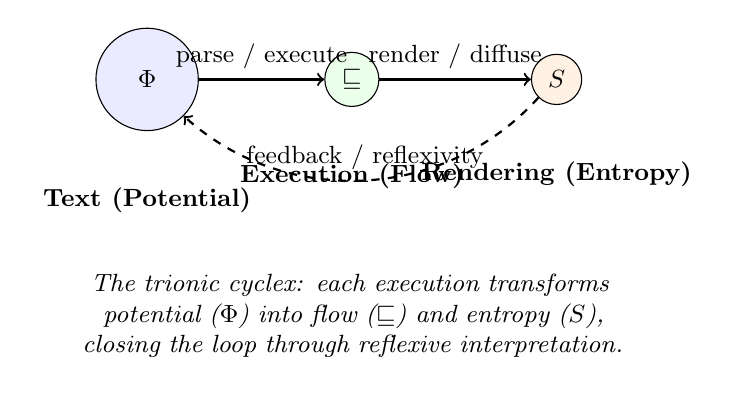
\begin{tikzpicture}[node distance=2.6cm, every node/.style={font=\small}]
\node (phi) [circle, draw, fill=blue!8, minimum width=1.3cm] {$\Phifield$};
\node (v) [circle, draw, fill=green!8, right of=phi] {$\vfield$};
\node (s) [circle, draw, fill=orange!10, right of=v] {$\Sfield$};

\draw[->, thick] (phi) -- (v) node[midway,above]{parse / execute};
\draw[->, thick] (v) -- (s) node[midway,above]{render / diffuse};
\draw[->, dashed, thick, bend left=45] (s) to node[midway,above]{feedback / reflexivity} (phi);

\node[below=0.6cm of phi] {\textbf{Text (Potential)}};
\node[below=0.6cm of v] {\textbf{Execution (Flow)}};
\node[below=0.6cm of s] {\textbf{Rendering (Entropy)}};

\node[below=2cm of v, align=center, text width=8cm]
{\textit{The trionic cyclex: each execution transforms potential ($\Phifield$) into flow ($\vfield$) and entropy ($\Sfield$), closing the loop through reflexive interpretation.}};
\end{tikzpicture}
\caption{Trionic cyclex and RSVP field coupling. Dashed arrow denotes reflexive feedback from entropy to potential.}
\label{fig:trionic-cyclex}
\end{figure}

\section{Worked Micro-Example: Probabilistic L-System}
\label{app:micro-example}

We illustrate the Assembly–Complexity–Entropy pipeline on a minimal, stochastic L-system that generates polyline images resembling a randomised Koch family.

\paragraph{Basis and composition.}
Fix a primitive basis $\mathcal{B}$ (atoms) and admissible joins (constructors):
\[
\mathcal{B}=\{\texttt{SYM}(F,+,-),~\texttt{RULE},~\texttt{AXIOM},~\texttt{ANGLE},~\texttt{LEN},~\texttt{ITER},~\texttt{DRAW},~\texttt{PROB}\}.
\]
Admissible joins: \texttt{RULE}$(LHS,~RHS,~\texttt{PROB}(p))$, \texttt{AXIOM}$(w_0)$, \texttt{ANGLE}$(\theta)$, \texttt{LEN}$(\ell)$, \texttt{ITER}$(n)$, \texttt{DRAW}$(\cdot)$.

\paragraph{Generator $P_n(p,\theta,\ell)$.}
Axiom $w_0=\texttt{F}$ and a single probabilistic production:
\[
\texttt{F}\;\xrightarrow{\;\;p\;\;}\;\texttt{F+F},\qquad
\texttt{F}\;\xrightarrow{\;1-p\;}\;\texttt{F-F}.
\]
After $n$ iterations, interpret the word by a standard turtle: \texttt{F} draws a segment of length $\ell$, \texttt{+} turns $+\theta$, \texttt{-} turns $-\theta$.

\paragraph{Assembly transcript (explicit, $n=3$).}
A minimal transcript $\tau_3$ (atoms $\in\mathcal{B}$, with implicit parentheses/delimiters):
\[
\small
\underbrace{\texttt{AXIOM}(\texttt{F})}_{1}\;
\underbrace{\texttt{RULE}(\texttt{F},\,\texttt{F+F},\,\texttt{PROB}(p))}_{2}\;
\underbrace{\texttt{RULE}(\texttt{F},\,\texttt{F-F},\,\texttt{PROB}(1-p))}_{3}\;
\underbrace{\texttt{ANGLE}(\theta)}_{4}\;
\underbrace{\texttt{LEN}(\ell)}_{5}\;
\underbrace{\texttt{ITER}(3)}_{6}\;
\underbrace{\texttt{DRAW}}_{7}.
\]
Thus, with our basis, $P_3$ is assembled in $n_\mathrm{joins}=7$ irreducible joins.

\paragraph{Assembly Index.}
\[
\AI\big(P_n(p,\theta,\ell)\big)\;=\; c_0 \;+\; \Big\lceil\log_2 n\Big\rceil,
\]
where $c_0$ counts fixed joins (\texttt{AXIOM}, two \texttt{RULE}s, \texttt{ANGLE}, \texttt{LEN}, \texttt{DRAW}). Hence $\AI$ grows only \emph{logarithmically} with iteration depth $n$.

\paragraph{Render-space entropy.}
Let $N_F(n)$ be the number of \texttt{F} symbols after $n$ iterations. Because each \texttt{F} is replaced by one of two length-2 words independently,
\[
N_F(n) \;=\; 2^n.
\]
Each \texttt{F}\,$\to$\,(\texttt{F+F} or \texttt{F-F}) is a Bernoulli($p$) branch contributing $H_2(p)$ bits (binary entropy). Assuming independent local choices, the number of distinct expansion histories is $2^{2^n}$ and the Shannon entropy of expansion paths is
\[
\Sfield_{\mathrm{render}}(n) = 2^{n}\,H_2(p) \quad\text{bits},\qquad H_2(p)=-p\log_2 p-(1-p)\log_2(1-p).
\]
Thus
\[
\frac{d}{dn}\Sfield_{\mathrm{render}}(n)\;=\;(\ln 2)\,2^{n} H_2(p)\;>\;0\quad\text{for}\;p\in(0,1),
\]
while $\frac{d}{dn}\AI\big(P_n\big)\sim 1/(n\ln 2)$, confirming the complexity–entropy inversion.

\paragraph{Numeric table (illustrative).}
Take $p=\tfrac{1}{2}$, $\theta=60^\circ$, $\ell=1$, $|\mathcal{B}|=8$, $c_0=6$. Then:
\[
\AI(P_n) \approx 6 + \lceil \log_2 n \rceil, \qquad
\Sfield_{\text{render}}(n) = 2^n \,\text{bits}.
\]
\begin{center}
\renewcommand{\arraystretch}{1.2}
\begin{tabular}{@{}rccc@{}}
\toprule
$n$ & $\AI(P_n)$ & $2^n$ branches & $\Sfield_{\text{render}}(n)$ [bits] \\
\midrule
1 & $7$ & $2$ & $2$ \\
2 & $8$ & $4$ & $4$ \\
3 & $8$ & $8$ & $8$ \\
4 & $8$ & $16$ & $16$ \\
5 & $9$ & $32$ & $32$ \\
\bottomrule
\end{tabular}
\end{center}

\section{Appendix F — Deterministic Contrast: The Koch Curve Generator}
\label{app:koch-example}

To complement the probabilistic L-system, consider a fully deterministic variant: the classic Koch curve generator.

\paragraph{Generator $Q_n(\theta,\ell)$.}
Basis $\mathcal{B}_\mathrm{det}=\{\texttt{SYM}(F,+,-),~\texttt{RULE},~\texttt{AXIOM},~\texttt{ANGLE},~\texttt{LEN},~\texttt{ITER},~\texttt{DRAW}\}$. Production rule:
\[
\texttt{F}\;\to\;\texttt{F+F--F+F}, \qquad w_0=\texttt{F}, \qquad \theta=60^\circ, \qquad \ell>0.
\]
After $n$ iterations, \texttt{DRAW} interprets the resulting string as a polyline.

\paragraph{Assembly Index and transcript.}
The transcript $\tau$ differs from Appendix~\ref{app:micro-example} only by a single deterministic \texttt{RULE}. Thus,
\[
\AI(Q_n) \;=\; c_0' + \Big\lceil \log_2 n \Big\rceil, \qquad c_0'\approx 5.
\]
Assembly depth still scales logarithmically with iteration count.

\paragraph{Render entropy.}
Because all expansions are deterministic, each \texttt{F} has exactly one successor; hence the symbolic expansion entropy vanishes:
\[
\Sfield_{\mathrm{render}}(n)\;=\;0, \qquad \frac{d\Sfield_{\mathrm{render}}}{dn}=0.
\]
Nonetheless, the geometric complexity of the render (measured by the Hausdorff dimension) grows nontrivially: $D_\mathrm{H} = \frac{\log 4}{\log 3} \approx 1.2619$.

\paragraph{Comparative summary.}
\begin{center}
\renewcommand{\arraystretch}{1.2}
\begin{tabular}{@{}rcccc@{}}
\toprule
$n$ & $\AI(Q_n)$ & $N_F(n)$ & $\Sfield_{\text{render}}(n)$ [bits] & $D_\mathrm{H}$ \\
\midrule
1 & $6$ & $4$ & $0$ & $1.2619$ \\
2 & $7$ & $16$ & $0$ & $1.2619$ \\
3 & $8$ & $64$ & $0$ & $1.2619$ \\
4 & $8$ & $256$ & $0$ & $1.2619$ \\
\bottomrule
\end{tabular}
\end{center}

\section{Appendix G — 3D Procedural Comparison: Sierpiński Tetrahedron}
\label{app:sierpinski-3d}

\paragraph{Deterministic generator $R^{(3)}_{\mathrm{det}}$.}
Start from a regular tetrahedron with edge length $L$. At each iteration $k\mapsto k{+}1$: compute midpoints, subdivide into $8$ sub-tetrahedra, retain $4$ corner tetrahedra. After $n$ iterations, $N_{\mathrm{det}}(n)=4^{n}$, edge length $L_n=L/2^{n}$.

\paragraph{Assembly Index.}
\[
\AI(R^{(3)}_{\mathrm{det}})=c_1+\lceil\log_2 n\rceil, \qquad c_1\approx 5.
\]

\paragraph{Geometric complexity.}
Hausdorff dimension $D_{\mathrm{H}}^{(3)}=2$.

\paragraph{Stochastic generator $R^{(3)}_{\mathrm{stoch}}(p)$.}
Retain each of $8$ sub-tetrahedra independently with probability $p$. Expected retained: $(8p)^n$. Render entropy:
\[
\Sfield_{\mathrm{render}}^{(3)}(n) =8^n\,H_2(p).
\]
Effective dimension: $D_{\mathrm{H}}^{(3)}(p)=\frac{\log (8p)}{\log 2}$.

\paragraph{Comparative summary.}
\begin{center}
\renewcommand{\arraystretch}{1.2}
\begin{tabular}{@{}lcccc@{}}
\toprule
Generator & $\AI$ scaling & $\Sfield_{\text{render}}$ growth & $D_{\mathrm{H}}$ & Behavior \\
\midrule
$R^{(3)}_{\mathrm{det}}$ & $\log n$ & $0$ & $2.000$ & Deterministic fractal surface \\
$R^{(3)}_{\mathrm{stoch}}(p)$ & $\log n$ & $\sim8^{n}H_2(p)$ & $\log_2(8p)$ & Random fractal cloud \\
\bottomrule
\end{tabular}
\end{center}

% =====================================================
\section*{Notation}
\addcontentsline{toc}{section}{Notation}
\begin{tabular}{ll}
$M$ & Linguistic manifold (configuration space) \\
$\Phifield : M \to \mathbb{R}$ & Scalar potential field \\
$\vfield : M \times \mathbb{R}_+ \to TM$ & Vector flow field \\
$\Sfield[\Phifield, \vfield]$ & Entropy functional \\
$\AI(P)$ & Assembly Index of program $P$ \\
$K(P)$ & Kolmogorov complexity \\
\end{tabular}

% =====================================================
\section*{Glossary}
\addcontentsline{toc}{section}{Glossary}

\begin{description}[leftmargin=2em,style=nextline]
\item[Plenum] Informational substrate undergoing internal differentiation.
\item[Linguistic Manifold] Configuration space of syntactic states of code.
\item[Semantic Curvature] Second derivative $\nabla^2\Phifield$, measuring change of meaning density.
\item[Reflexivity] System’s inclusion of its own rules within representation.
\item[Computational Realism] View that executions are physically instantiated causal processes.
\item[Causal Depth] Historical assembly steps needed to reach a structure; measured by $\AI$.
\end{description}

% =====================================================
\section*{List of Formal Statements}
\addcontentsline{toc}{section}{List of Formal Statements}

\begin{itemize}
  \item \textbf{Definition 1.1} (Linguistic Manifold) — Sec.~\ref{sec:text-generator}
  \item \textbf{Eq. \eqref{eq:execution-sde}} (Stochastic Execution) — Sec.~\ref{sec:field-flow}
  \item \textbf{Theorem 4.1} (Compression–Entropy Bound) — Sec.~\ref{sec:compression-meaning}
  \item \textbf{Proposition 5.1} (Entropy Trade) — Sec.~\ref{sec:assembly-entropy}
  \item \textbf{Definition 8.1} (Attentional Fidelity) — Sec.~\ref{sec:automation-ethics}
  \item \textbf{Conjecture B.1} (Cognitive Conservation Law) — App.~\ref{app:phenomenology}
  \item \textbf{Theorem 12.1} (Functorial Structure) — Sec.~\ref{sec:objections}
  \item \textbf{Proposition 2.3} (SDE Existence) — Sec.~\ref{sec:field-flow}
  \item \textbf{Theorem 6.1} (Second Law for Code) — Sec.~\ref{sec:rendering-entropy}
  \item \textbf{Theorem 8.1} (P vs Curvature) — Sec.~\ref{sec:complexity}
\end{itemize}

% =====================================================
\section*{Acknowledgments}
\addcontentsline{toc}{section}{Acknowledgments}

Thanks to the command line, to modal editors, to hotkeys and shells— the instruments by which law becomes motion. Every keystroke in \texttt{vim} bends $\Phifield$; every multiplexed pane propagates $\vfield$; every saved artifact diffuses into $\Sfield$. May recursion remain bounded by awareness.

% =====================================================
\begin{thebibliography}{12}
\addcontentsline{toc}{section}{References}

\bibitem{Cronin2023}
L.~Cronin et al. (2023). ``The Assembly Theory of Matter.'' \emph{Nature} 623: 53–60.

\bibitem{Kolmogorov1965}
A.~N. Kolmogorov (1965). ``Three Approaches to the Definition of the Quantity of Information.'' \emph{Problems of Information Transmission} 1(1): 1–7.

\bibitem{Chaitin2007}
G.~J. Chaitin (2007). \emph{Meta Math! The Quest for Omega.} Pantheon.

\bibitem{Wheeler1990}
J.~A. Wheeler (1990). ``Information, Physics, Quantum: The Search for Links.'' In \emph{Proc. 3rd Int. Symp. on Foundations of Quantum Mechanics.}

\bibitem{Lloyd2006}
S.~Lloyd (2006). \emph{Programming the Universe: A Quantum Computer Scientist Takes on the Cosmos.} Knopf.

\bibitem{LadymanRoss2007}
J.~Ladyman \& D.~Ross (2007). \emph{Every Thing Must Go: Metaphysics Naturalized.} Oxford UP.

\bibitem{Floridi2011}
L.~Floridi (2011). \emph{The Philosophy of Information.} Oxford UP.

\bibitem{DeLanda2002}
M.~DeLanda (2002). \emph{Intensive Science and Virtual Philosophy.} Continuum.

\bibitem{Tegmark2014}
M.~Tegmark (2014). \emph{Our Mathematical Universe.} Knopf.

\bibitem{CroninBound2024}
L.~Cronin \& S.~Marshall (2024). ``Causal Depth and Life Detection.'' \emph{Science Advances} 10(3): eaay8254.

\bibitem{PrintScreen}
\texttt{PrintScreen.ahk} (2025). AutoHotkey script for reflexive capture. Available at \url{https://github.com/standardgalactic/example/blob/volsorium/PrintScreen.ahk}.

\end{thebibliography}

\printindex
\end{document}
